\graphicspath{{./Figs/}}

\chapter{Theory and Methodology}
This chapter outlines the theory and methodology used to create, test and collect the data required for the wing-propeller interaction analysis. It covers the development of the \acrshort{MAV} model for testing from python scripts and FreeCAD to the final testing completed in a 3x4ft wind tunnel to collect the force and moment data of the model. The software used to validate these results is also explained in this chapter. 

\section{Material Choice}
To readily edit and modify the model to be tested, 3D printing was used to print the final developed model. 3D printing has become increasingly common when developing models testing in wind tunnels \cite{Szwedziak2022}. Polylactic acid (\acrshort{PLA}) filament was used to print the main body of the model as this is the most widely used and available filament for 3D printing purposes. \acrshort{PLA} has a low melting point of $\approx$ 150 $^{\circ}$, good layer adhesion and structural strength. \acrshort{PLA} can also be extruded in various ways to develop different textures on the surface of the 3D model \cite{Butt2021}. This is particularly significant for \acrshort{MAV}s as aircraft surfaces are typically smooth to reduce viscous drag effects. 3D printed models may have thin ridges between layers when printed. However, the extrusion rate, nozzle size, temperature, and bed temperature can all be set to mitigate this issue as much as possible \cite{Butt2021} \cite{Olasek2014}. However, a lightweight \acrshort{PLA} was used for the wings and tail to print a smoother surface. This is particularly important for the wings and tail as these are the main surfaces that provide lift for the aircraft. Using a lightweight \acrshort{PLA}, the structure allows for some bending, as seen in typical wing shapes, rather than printing with standard \acrshort{PLA} to produce a rigid structure. 


\section{FreeCAD}
FreeCAD is a 3D parametric modeller and was used with python scripts provided by Dries Verstraete to produce fuselage, wing and tail shapes when given input parameters to define the shape and geometry. Various model shapes were produced to make the model 3D printable and allow for easy manufacturing and testing. Several design constraints had to be considered due to the structural strength of the PLA used for 3D printing and size limitations. The wings and tail in particular had to be large enough to print the aerofoil shape accurately.  The TL54 airfoil was used for the main wings due to this airfoil having a high lift coefficient and low pitching moment. The model's dimensions are also given in Figure \ref{fig:dimension22}. The model shown in Figure \ref{fig:freeCADModel} was also fitted to mount into the 3x4ft wind tunnel for testing as shown in Figure \ref{fig:modelWithTunnel}.


\begin{figure}[H]
\centering
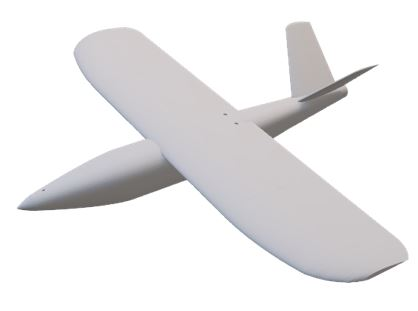
\includegraphics[]{04_Methodology/Figs/model2.jpg}
\caption{Final model for wind tunnel testing in FreeCAD}
\label{fig:freeCADModel}
\end{figure}


\begin{figure}
    \centering
    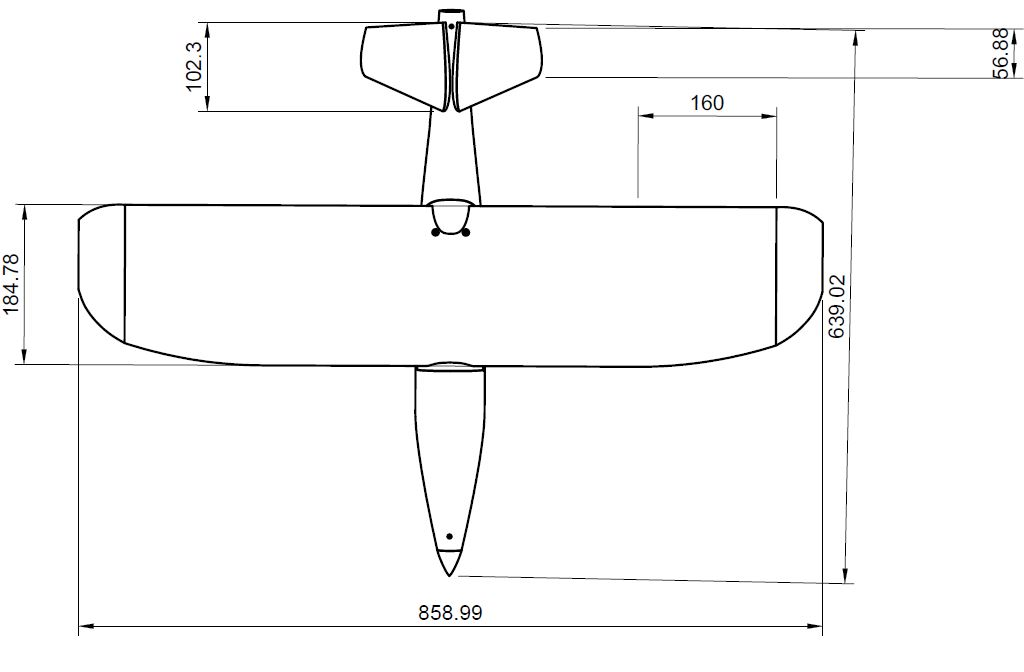
\includegraphics{04_Methodology/Figs/dimensions.JPG}
    
    \caption{Dimensions of the final \acrshort{MAV} model in millimeters}
    \label{fig:dimension22}
\end{figure}





\begin{figure}
    \centering
    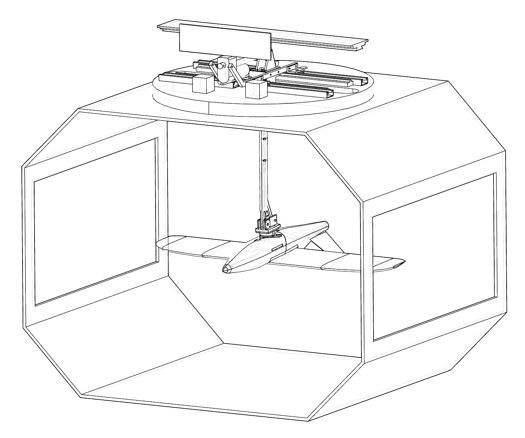
\includegraphics{04_Methodology/Figs/ModelWithtunnel.JPG}
    \caption{FreeCAD model mounted in Wing tunnel }
    \label{fig:modelWithTunnel}
\end{figure}

The model size was chosen to reduce the blockage experienced when using the model during wind tunnel testing. The blockage varied from 4.9\% to 8.7\% for an angle of attack range from -5$^\circ$ to 15$^\circ$. The wing span was also limited in size to ensure that wind tunnel interference would not influence the results. 



\section{VAP 3.5}
VAP 3.5 is open-source software that uses the High-Order Free Wake (\acrshort{HOFW}) method to determine the aerodynamic performance of \acrshort{MAV} designs. \\

The software is used by first defining the flight conditions and geometry of the model to be tested. This includes setting the duration of the simulation to ensure that the wake from the propeller and wing have interacted and fully developed. The VAP 3.5 model is then generated and run through the potential flow method used by the VAP 3.5 software. This is used to determine the aerodynamics of the \acrshort{MAV} design to be tested. The weight and \acrshort{CG} location of the model as determined based on the \acrshort{MAV} geometry or explicitly defined in the code used to generate the model. The stability derivatives can be determined based on the \acrshort{CG} location and the lift distribution determined in the VAP 3.5 potential flow method. A flowchart is given in Figure \ref{fig:flowchart} to outline this process.

 
 \begin{figure}[!ht]
 \centering
 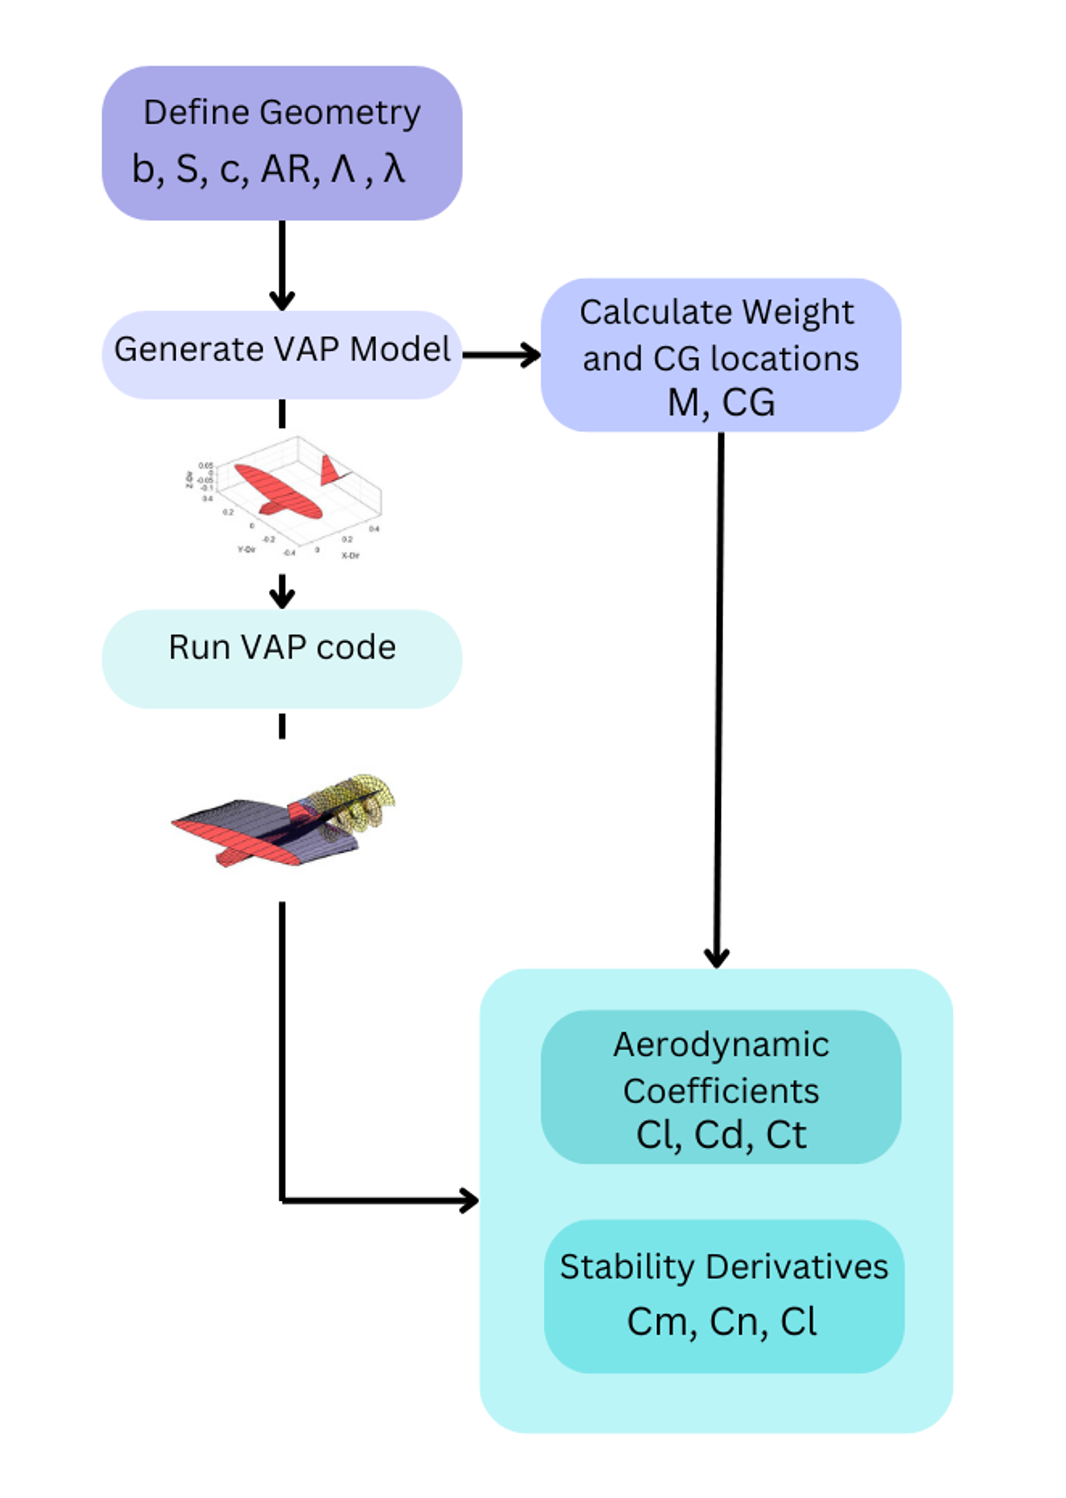
\includegraphics[scale=0.6]{04_Methodology/Figs/jasmine.png}
 \caption{VAP 3.5 main steps to setup, run and return results from simulation}
 \label{fig:flowchart}
 \end{figure}



The \acrshort{HOFW} method uses higher-order vorticity elements to represent the wings and propeller blades as lifting surfaces. This method has a faster computational speed, numerical stability and realistic prediction than alternatives such as the Navier-Stokes equations, fixed wake panel method, relaxed wake method or the Vortex Lattice Method (\acrshort{VLM}). It was initially developed to create a potential flow method that allowed for improved force resolution and intrinsic computational stability while keeping a simple geometric representation \cite{Cole2019}. This method has also been shown to be suitable for lightly loaded propeller/proprotors and propeller-wing systems. The \acrshort{HOFW} method is a higher-order, relaxed-wake potential flow method which imposes Neumann boundary conditions. It consists of a non-linear vorticity distribution along the transverse and linear distribution along the streamwise edges of a single Distributed Vortex Element (\acrshort{DVE}). A single element is shown in figure \ref{fig:Votices}. 

\begin{figure}
\centering
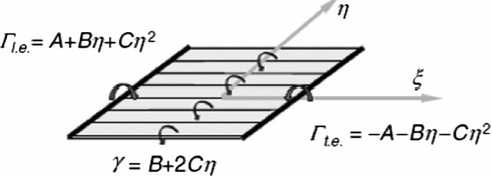
\includegraphics[width=0.7\linewidth]{04_Methodology/Figs/votex.png}
\caption{Visualisation of a single distributed vorticity element. The leading and trailing edge vortices are represented by $\Gamma_{l.e}$ and $\Gamma_{t.e}$, respectively. The quadratic circular distribution is in the spanwise $\eta$ direction, and the leading and trailing edge vortices are joined in the streamwise direction by a linear changing distribution vorticity strength indicated by $\gamma$ in the spanwise direction \cite{Cole2019}.}
\label{fig:Votices}
\end{figure}

For propeller-wing systems, the circulation distribution over each surface distributed vorticity element (\acrshort{SDVE}) is calculated using Equation \ref{eqn:vor}. Where [A] is the influence matrix which is a function of the geometry representing the lifting surfaces, \{x\} is a vector of the unknown DVE strengths, and \{B\} is the resultant vector where the boundary conditions are applied. A, B, and C hence represent the coefficients of the circulation distribution.

\begin{equation}
[A]\{x\} = \{B\}
\label{eqn:vor}
\end{equation}

The transverse vorticity axis ($\eta$) uses a quadratic function to model the vorticity distribution, whereas the streamwise axis ($\zeta$) uses a linear process. The simplicity allows for ease of calculation compared to alternative methods. The total force due to the lift of each \acrshort{SDVE} is the summation of the kinematic velocity and the force calculated with the induced velocity as given by Equation \ref{eqn:lift22} \cite{Cole2019}.

\begin{equation}
{\overline{F}}_{total} = \overline{F}_k + \overline{F}_{ind}
\label{eqn:lift22}
\end{equation}

The kinematic lift force and induced velocity force are determined at each time step to determine the lift and drag as they are defined relative to the freestream velocity. The kinematic lift force is calculated using Equation \ref{eqn:kinematic}

\begin{equation}
\overline{F}_k = \rho \sum_{i=1}^{m} \sum_{j=1}^{n} \left[ \int_{-\eta_{i,j}}^{\eta_{i,j}} |\overline{V}_k \times  \hat{s_{i,j}} | (\Gamma_{i,j} - \Gamma_{i-1,j}d\eta \frac{ \overline{V}_k \times \hat{s_{i,j}} }{|\overline{V}_k \times \hat{s_{i,j}|}} \right]
\label{eqn:kinematic}
\end{equation}

Where n is the number of spanwise panels, m is the number of lifting lines, $\eta$ is the half span and $\hat{s}$ is the unit vector along the leading-edge bound vortex of the distributed vorticity element. The induced velocity forces are calculated using Equation \ref{eqn:induced}.

\begin{equation}
\overline{F}_{ind} = \rho \sum_{i=1}^{m} \sum_{j=1}^{n} \left[ \int_{-\eta_{i,j}}^{\eta_{i,j}} |\overline{V}_{ind} \times  \hat{s_{i,j}} | (\Gamma_{i,j} - \Gamma_{i-1,j}d\eta \left(\frac{ \overline{V}_{ind} \times \hat{s_{i,j}} }{|\overline{V}_{ind} \times \hat{s_{i,j}|}}\right) \cdot \left(\frac{ \overline{V}_k \times \hat{s_{i,j}} }{|\overline{V}_k \times \hat{s_{i,j}|}}\right) \right]
\label{eqn:induced}
\end{equation}






\section{XFOIL}
XFOIL, developed by Harold Youngren and Mark Drela was used to analyse 2D airfoils for their aerodynamic characteristics. XFOIL was used to produce aerofoil data which accounted for viscous effects.  Viscous effects have an essential role in the flow characteristics across the surface of an aircraft wing. This is particularly important at lower Reynolds numbers. Xfoil uses the wake momentum thickness to determine the skin friction produced as the fluid passes over the airfoil surface as given by Equation \ref{eqn:XFOIL}. In this manner the skin friction losses can be determined and accounted for when running the VAP 3.5 software to analyse the stability of the model. 



\begin{equation}
    \theta = \int_{0}^{\infty} \frac{u}{U_e} ( 1 - \frac{u}{U_e) } \,dy
    \label{eqn:XFOIL}
\end{equation}

Where:
\begin{itemize}
    \item $\theta$ is the momentum thickness at a given point along the airfoil
    \item $U_e$ is the freestream velocity 
    \item u is the flow velocity at a position y distance from the airfoil surface
\end{itemize}


\section{Wind Tunnel Testing}
To analyse the stability of the final developed model, the model was mounted in the 3x4 ft wind tunnel to determine the forces and moments acting at several conditions to assess the effect that adding a propeller has on the stability of the model. Wind tunnel tests were taken for variations of \acrshort{AoA}, airspeed, propeller speed and configuration. These are outlined below

\begin{itemize}
    \item \acrshort{AoA}: -5 $^{\circ}$ to 15 $^{\circ}$ in increments of 2$^{\circ}$
    \item Airspeed: 10m/s, 15m/s and 20m/s
    \item Motor speed: 6000RPM, 9000RPM, 11000RPM
    \item Configuration: No propeller, tractor and pusher
\end{itemize}


A safety net was placed in the wind tunnel in case parts of the model could not remain attached as the airspeed increased to 20m/s, as shown in Figure \ref{fig:windTunnelNet}. An external cooler was used to ensure that the wind tunnel motor did not overheat and is shown in Figure \ref{fig:engineCooler}.

% \begin{figure}[H]
% \centering
% \begin{subfigure}[b]{0.3\textwidth}
%     \centering
%     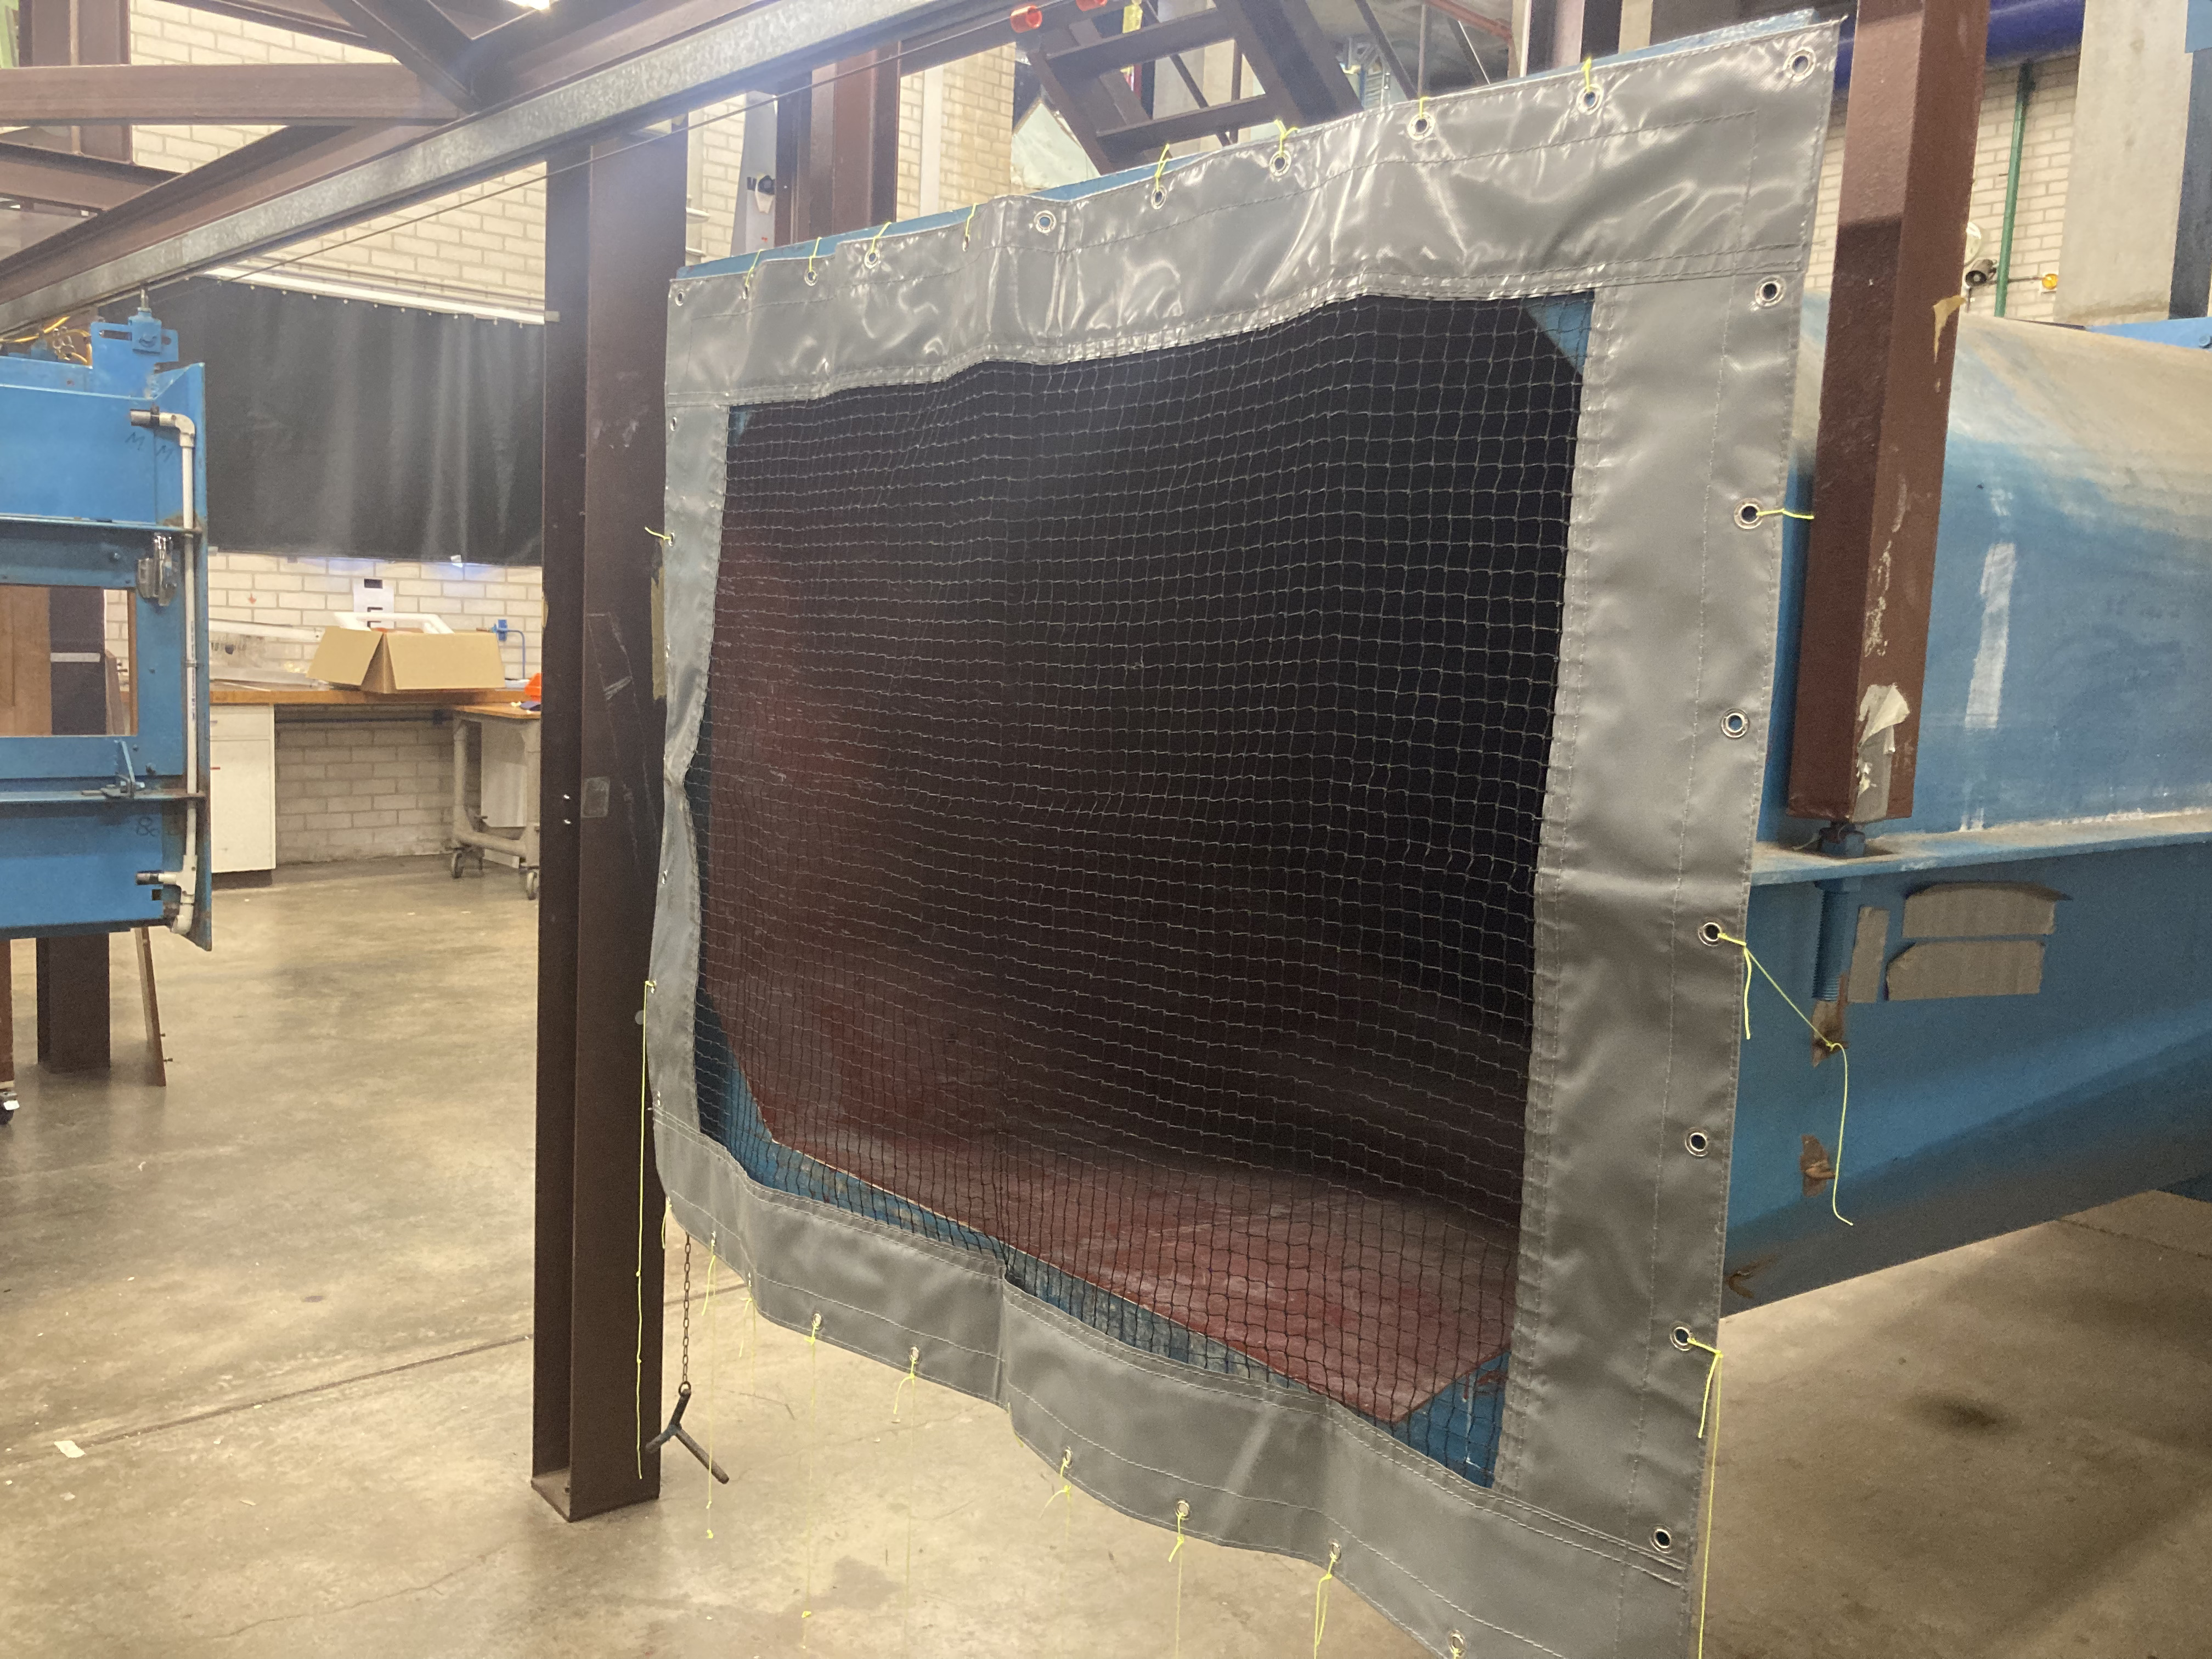
\includegraphics[scale =0.05]{04_Methodology/Figs/windTunnelNet.jpg}
%     \caption{Safety net to prevent any model parts from damaging the wind tunnel if the mount were to disconnect}
%     \label{fig:windTunnelNet}
% \end{subfigure}

% \hfill
% \begin{subfigure}[b]{0.3\textwidth}
%      \centering
%     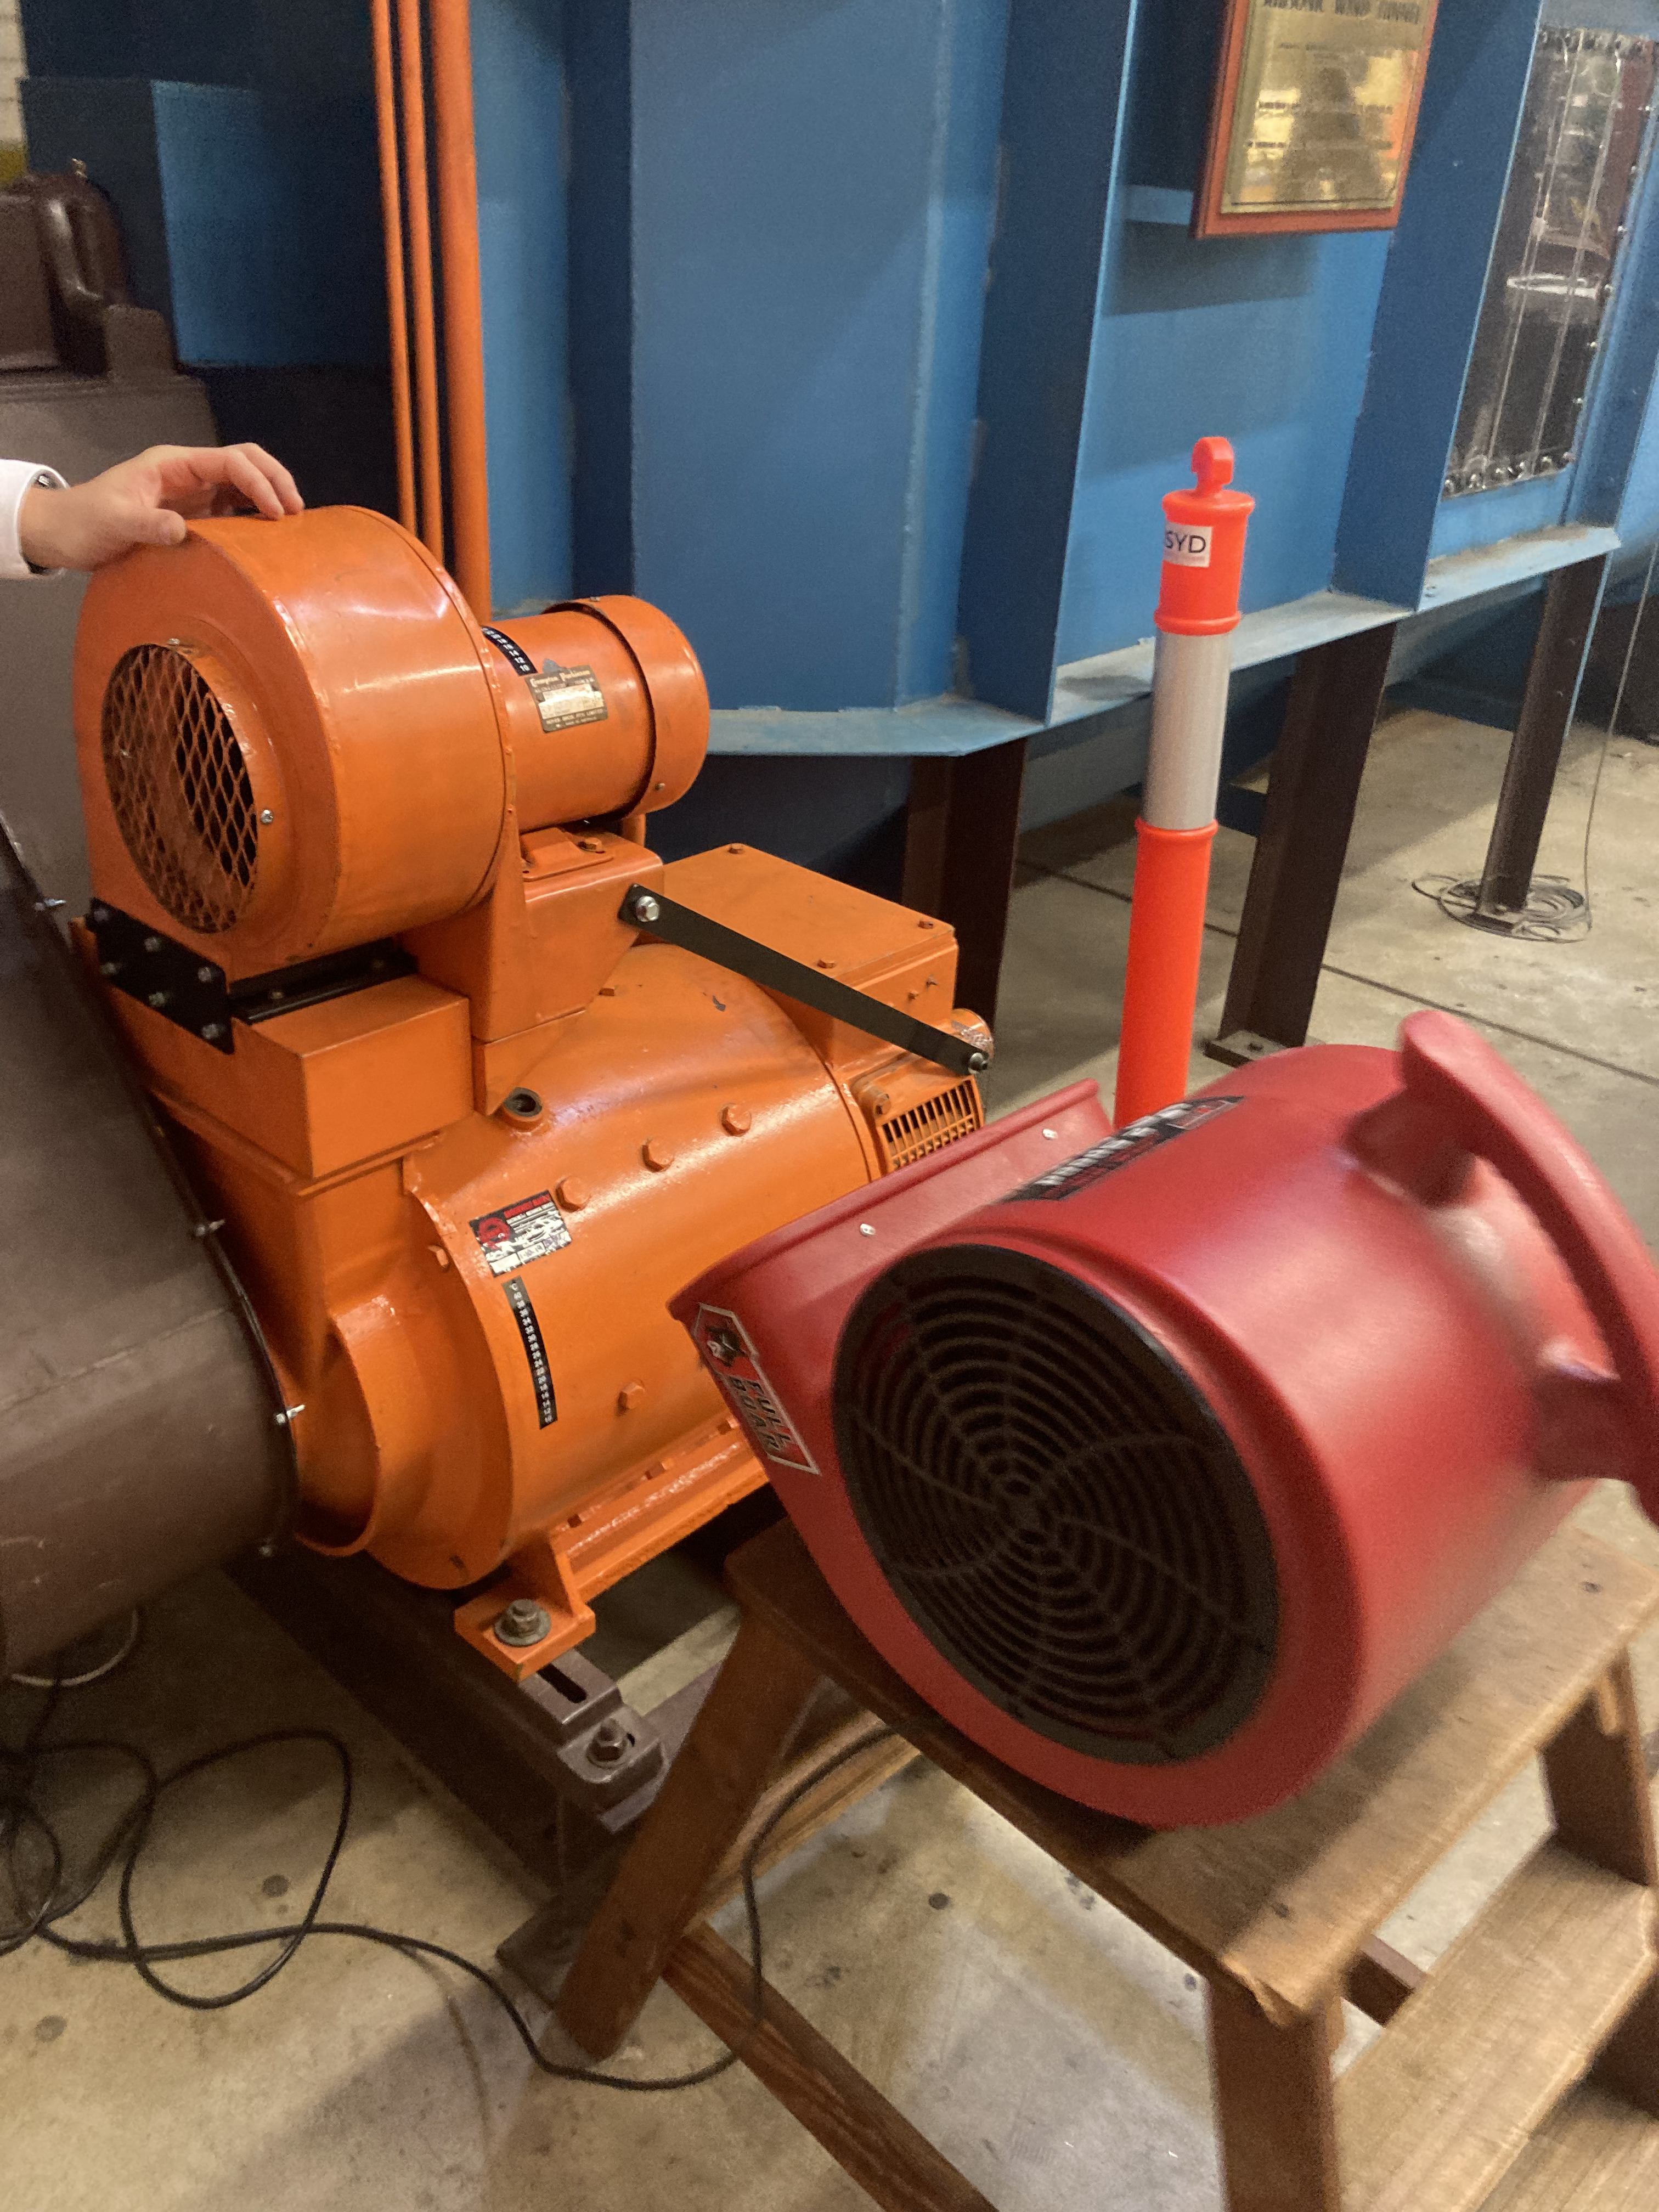
\includegraphics[scale=0.05]{04_Methodology/Figs/cooler.jpg}
%     \caption{Cooler for wind tunnel engine}
%     \label{fig:engineCooler}
% \end{subfigure}
% \hfill
    
% \end{figure}


\begin{figure}[H]
     \centering
     \begin{subfigure}[b]{0.4\textwidth}
             \centering
            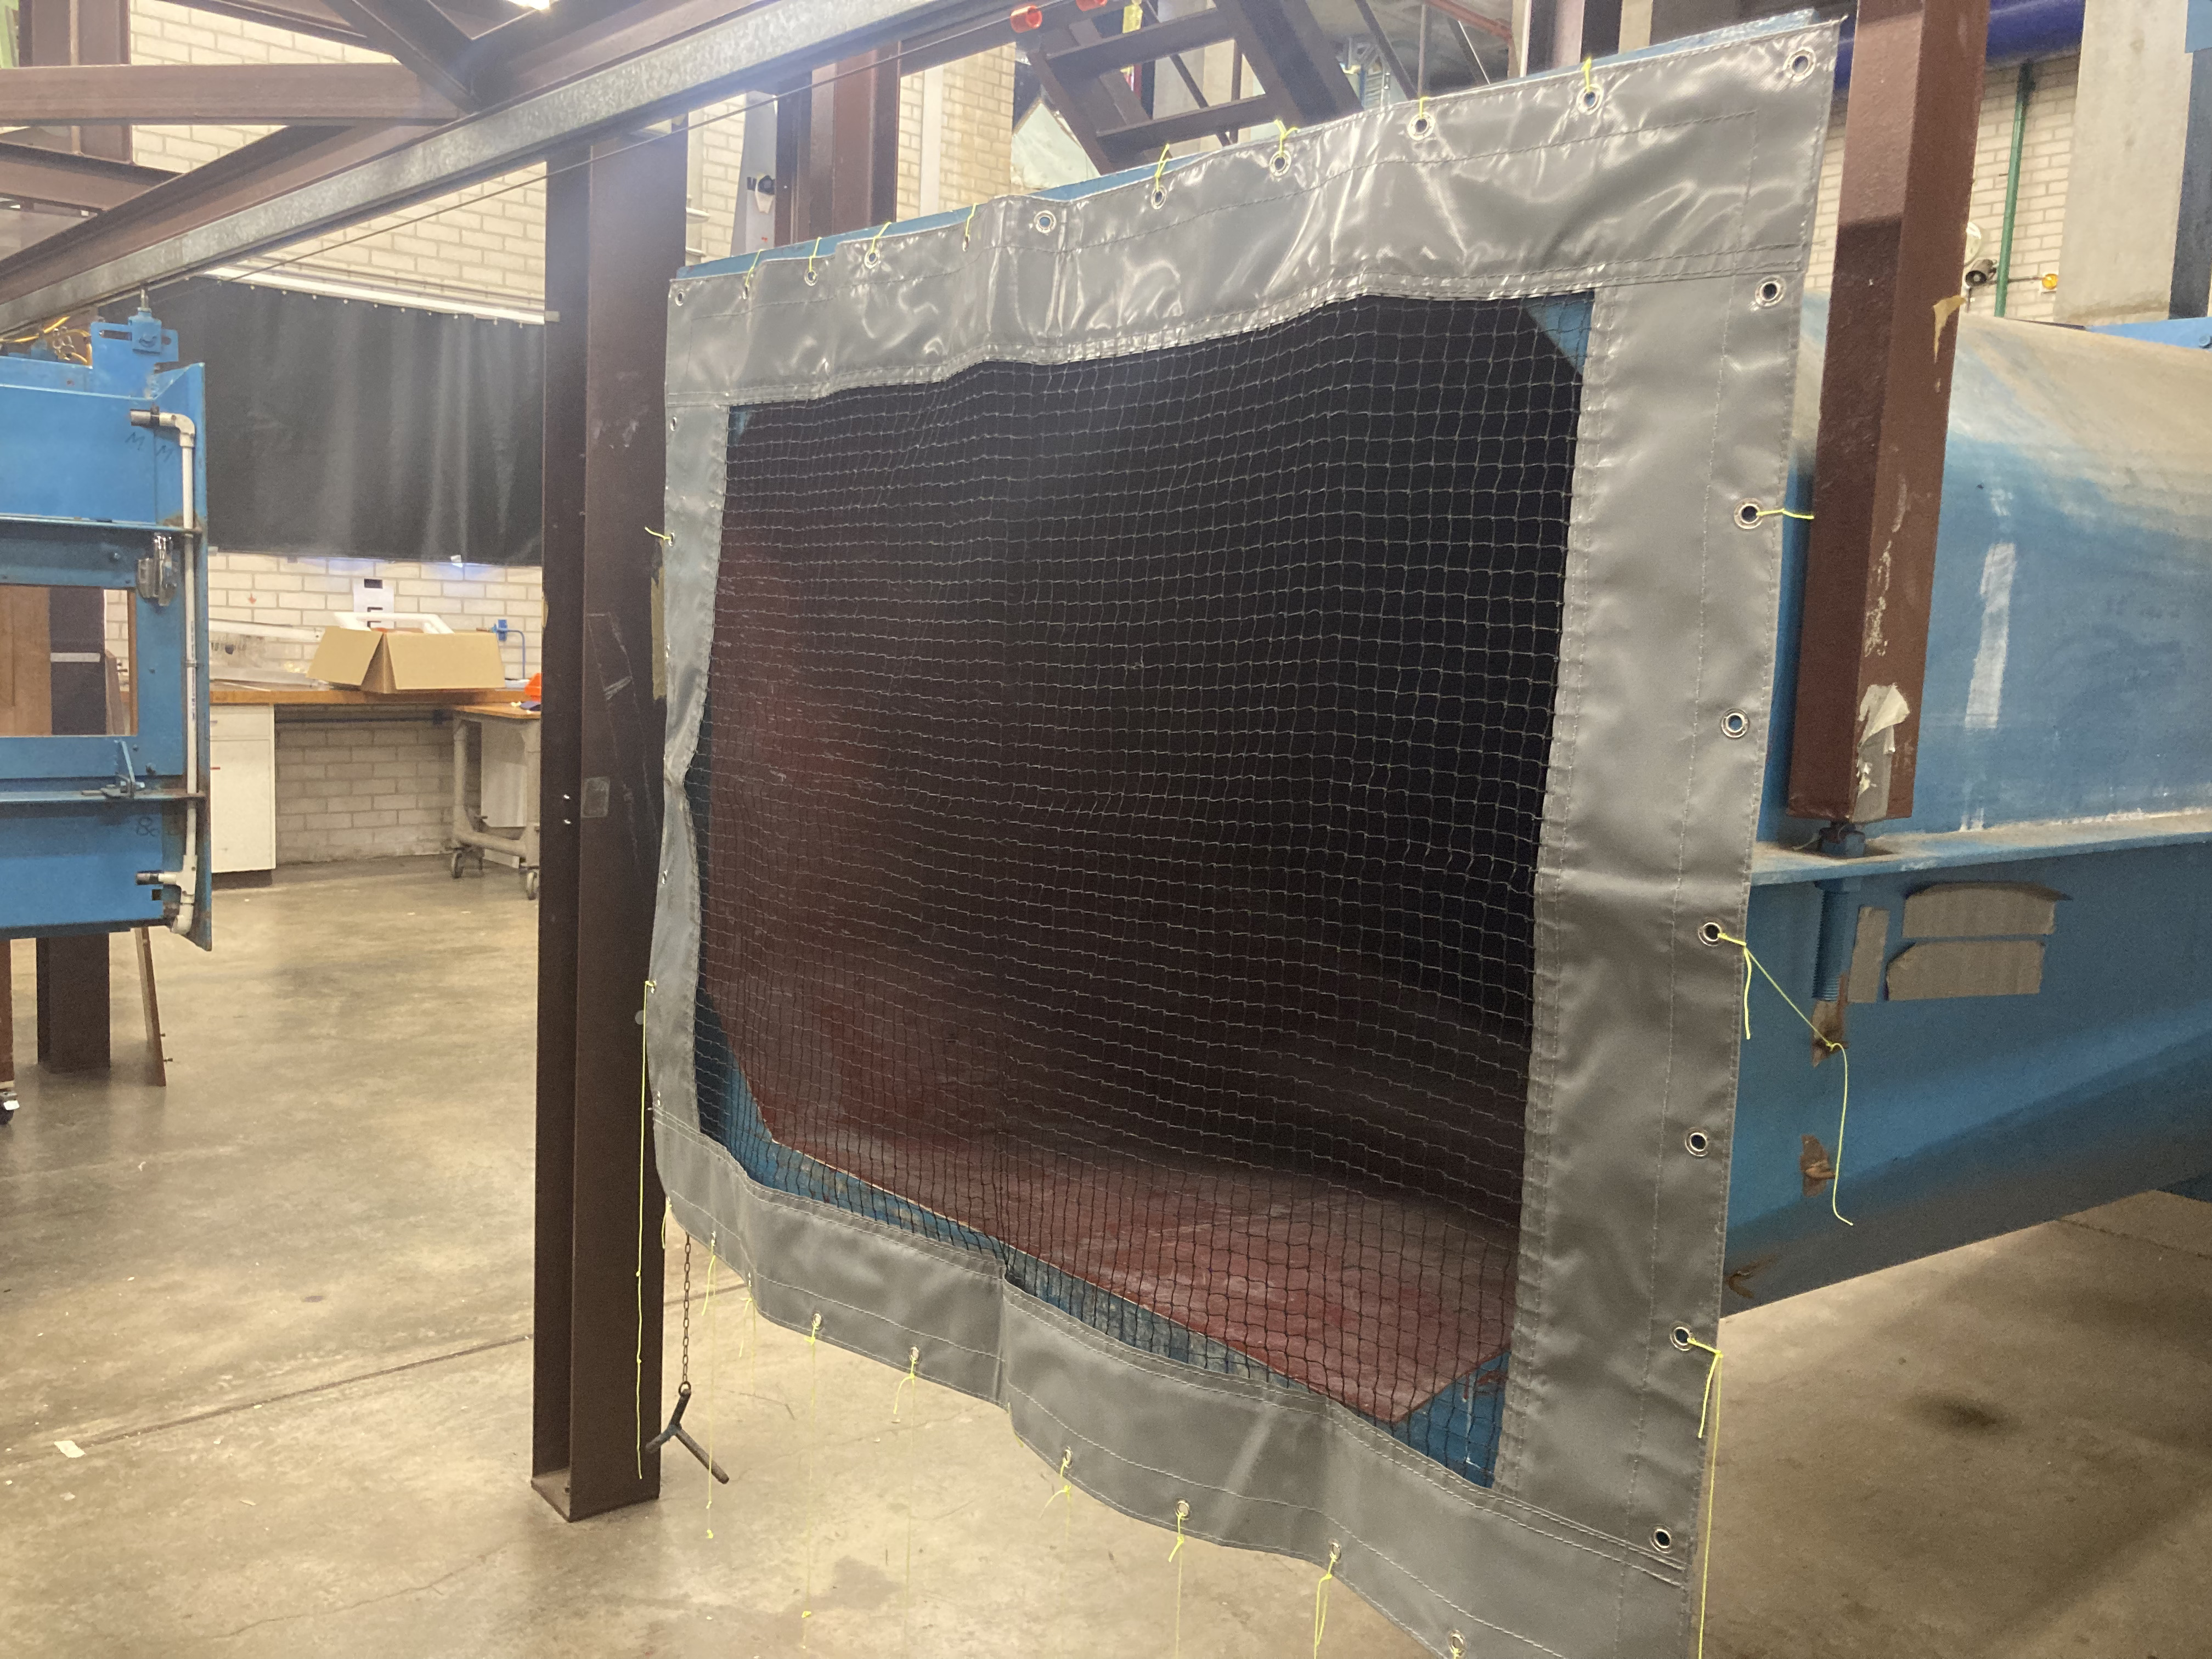
\includegraphics[scale =0.04]{04_Methodology/Figs/windTunnelNet.jpg}
            \caption{Safety net to prevent any model parts from damaging the wind tunnel if the mount were to disconnect}
            \label{fig:windTunnelNet}
     \end{subfigure}
     \hfill
     \begin{subfigure}[b]{0.4\textwidth}
                \centering
                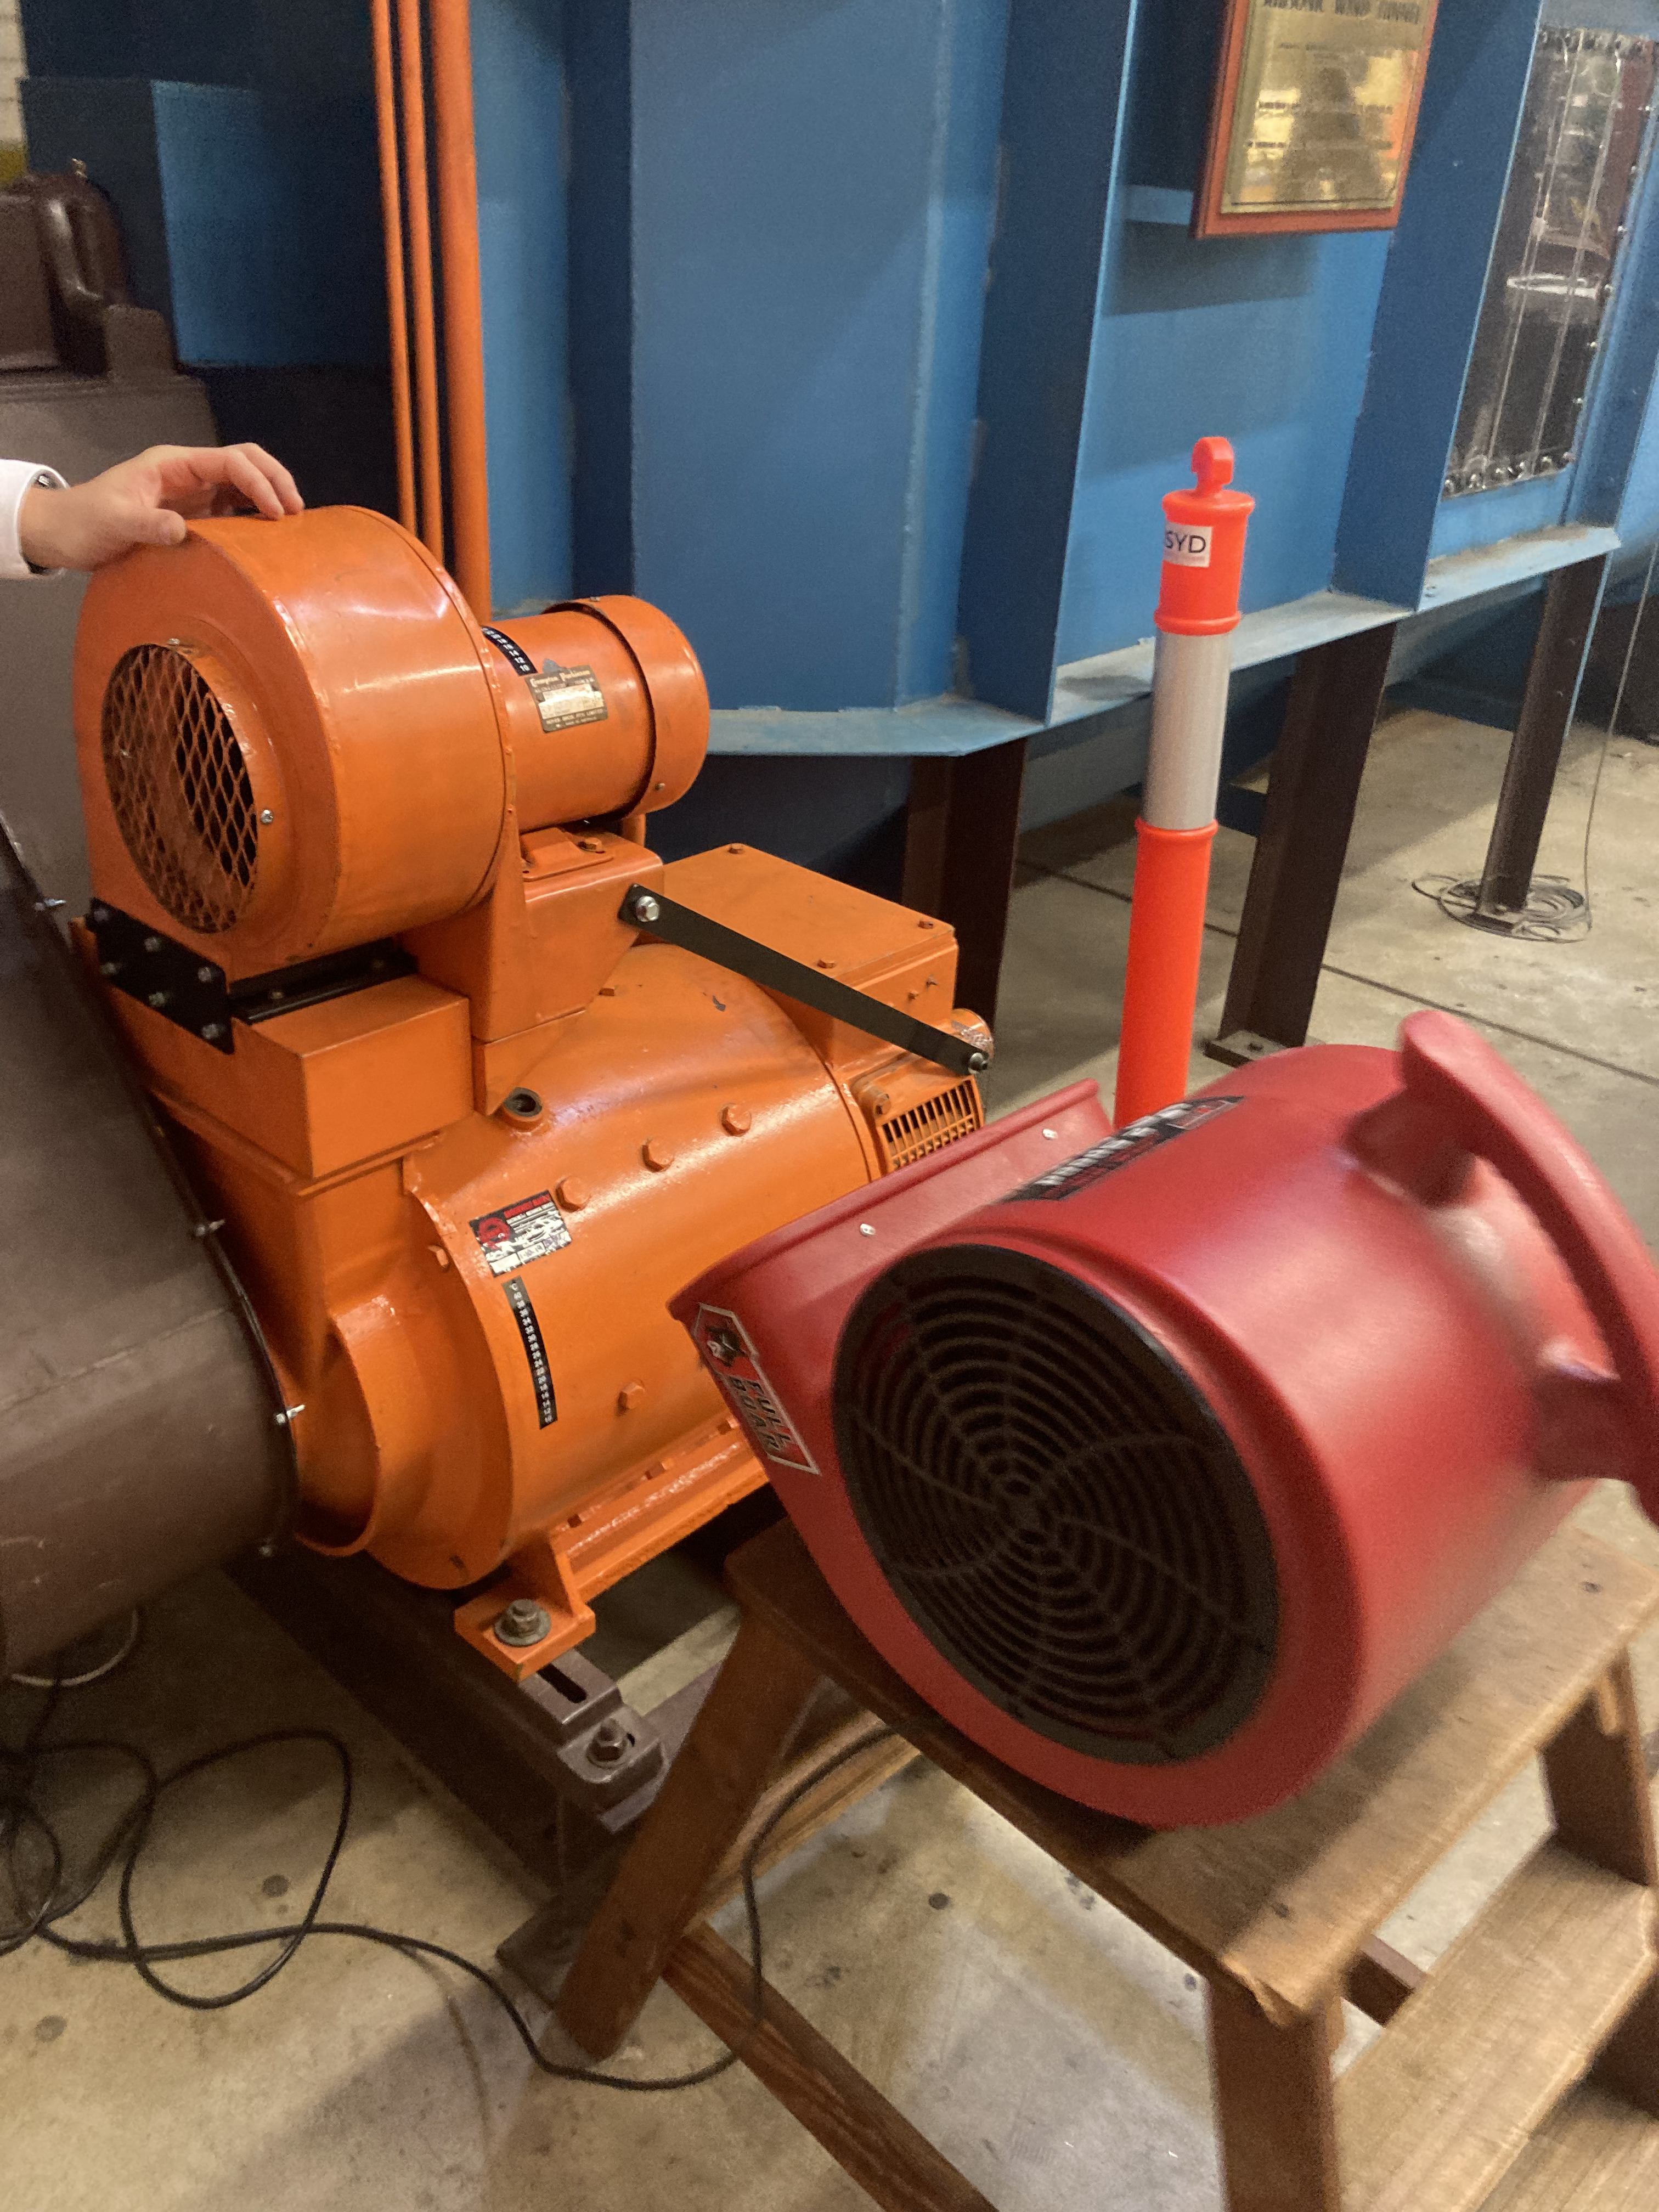
\includegraphics[scale=0.04]{04_Methodology/Figs/cooler.jpg}
                \caption{Cooler for wind tunnel motor}
                \label{fig:engineCooler}
     \end{subfigure}
     \caption{Safety measures taken to ensure no damage is done to any people or to the wind tunnel itself.}
     \label{fig:windTunnelSafety}
\end{figure}

% \begin{figure}[H]
%     \centering
%     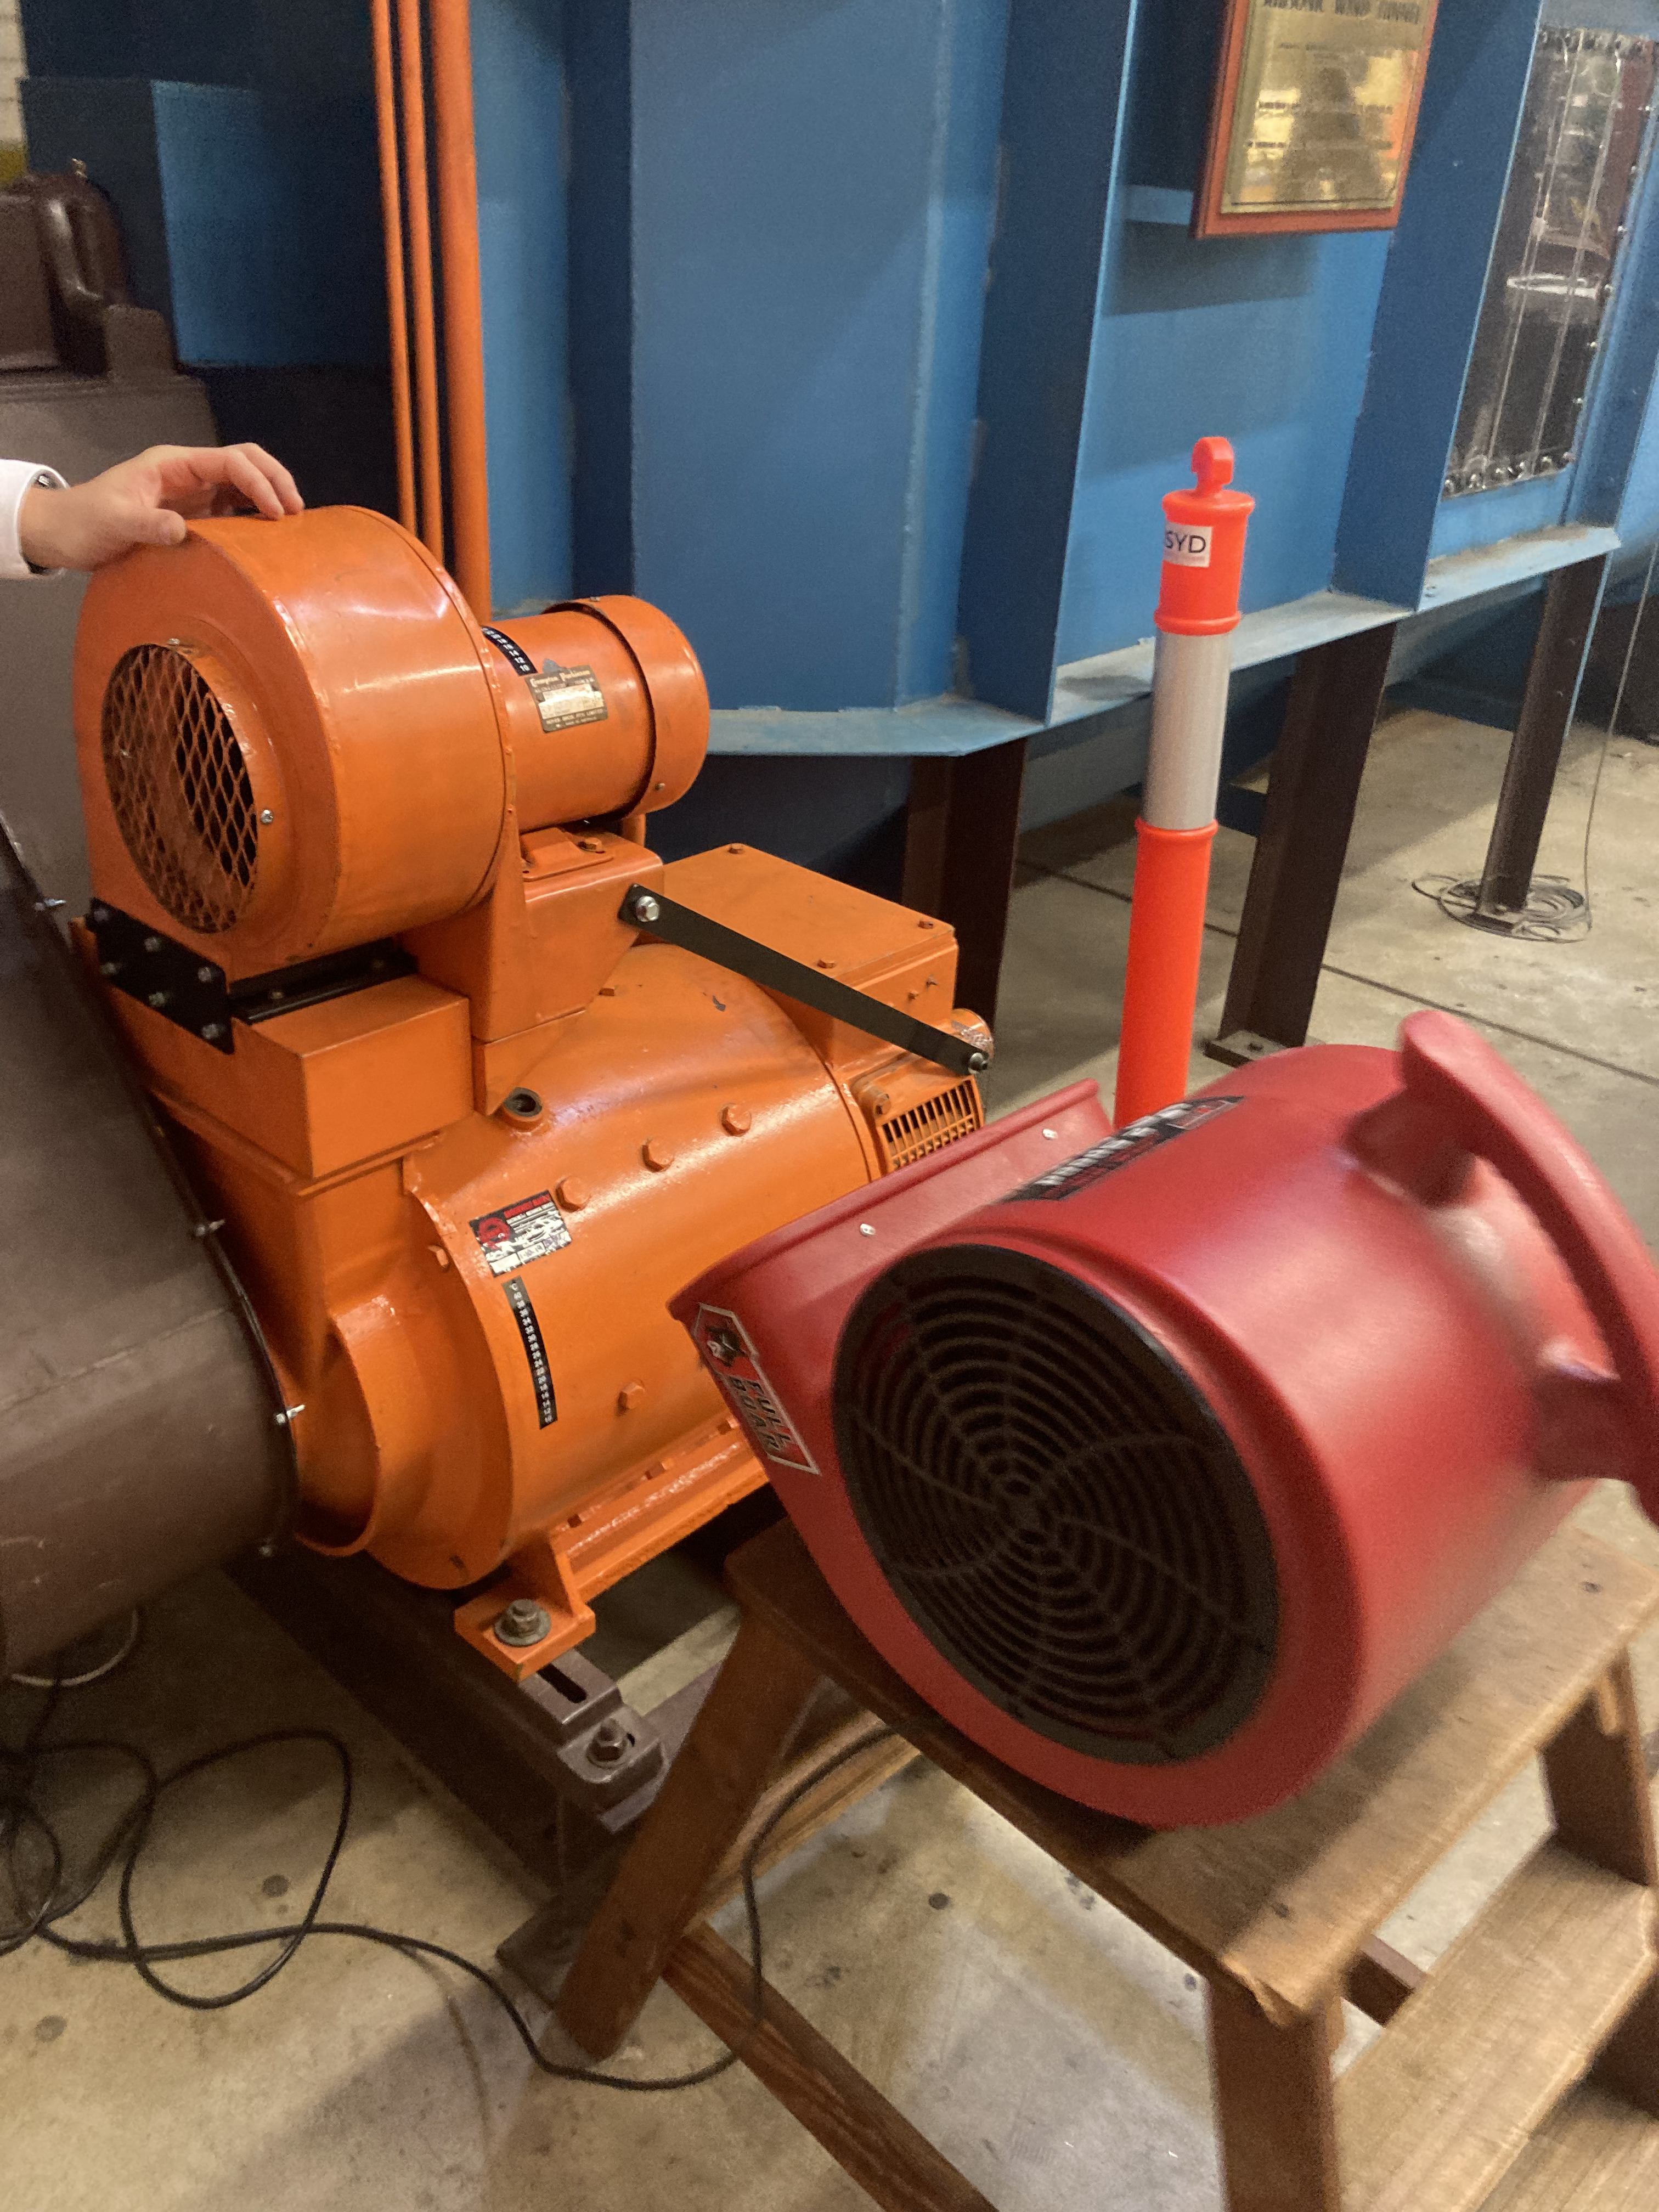
\includegraphics[scale=0.1]{04_Methodology/Figs/cooler.jpg}
%     \caption{Caption}
%     \label{fig:engineCooler}
% \end{figure}

The nano25 load cell was used to record the forces and moments acting on the model about the mounting position at 25$\overline{c}$ and is shown in Figure \ref{fig:LoadCella}. The model mount was then attached over the load cell as shown in Figure \ref{fig:LoadCellb}

\begin{figure}[H]
     \centering
     \begin{subfigure}[b]{0.45\textwidth}
               \centering
                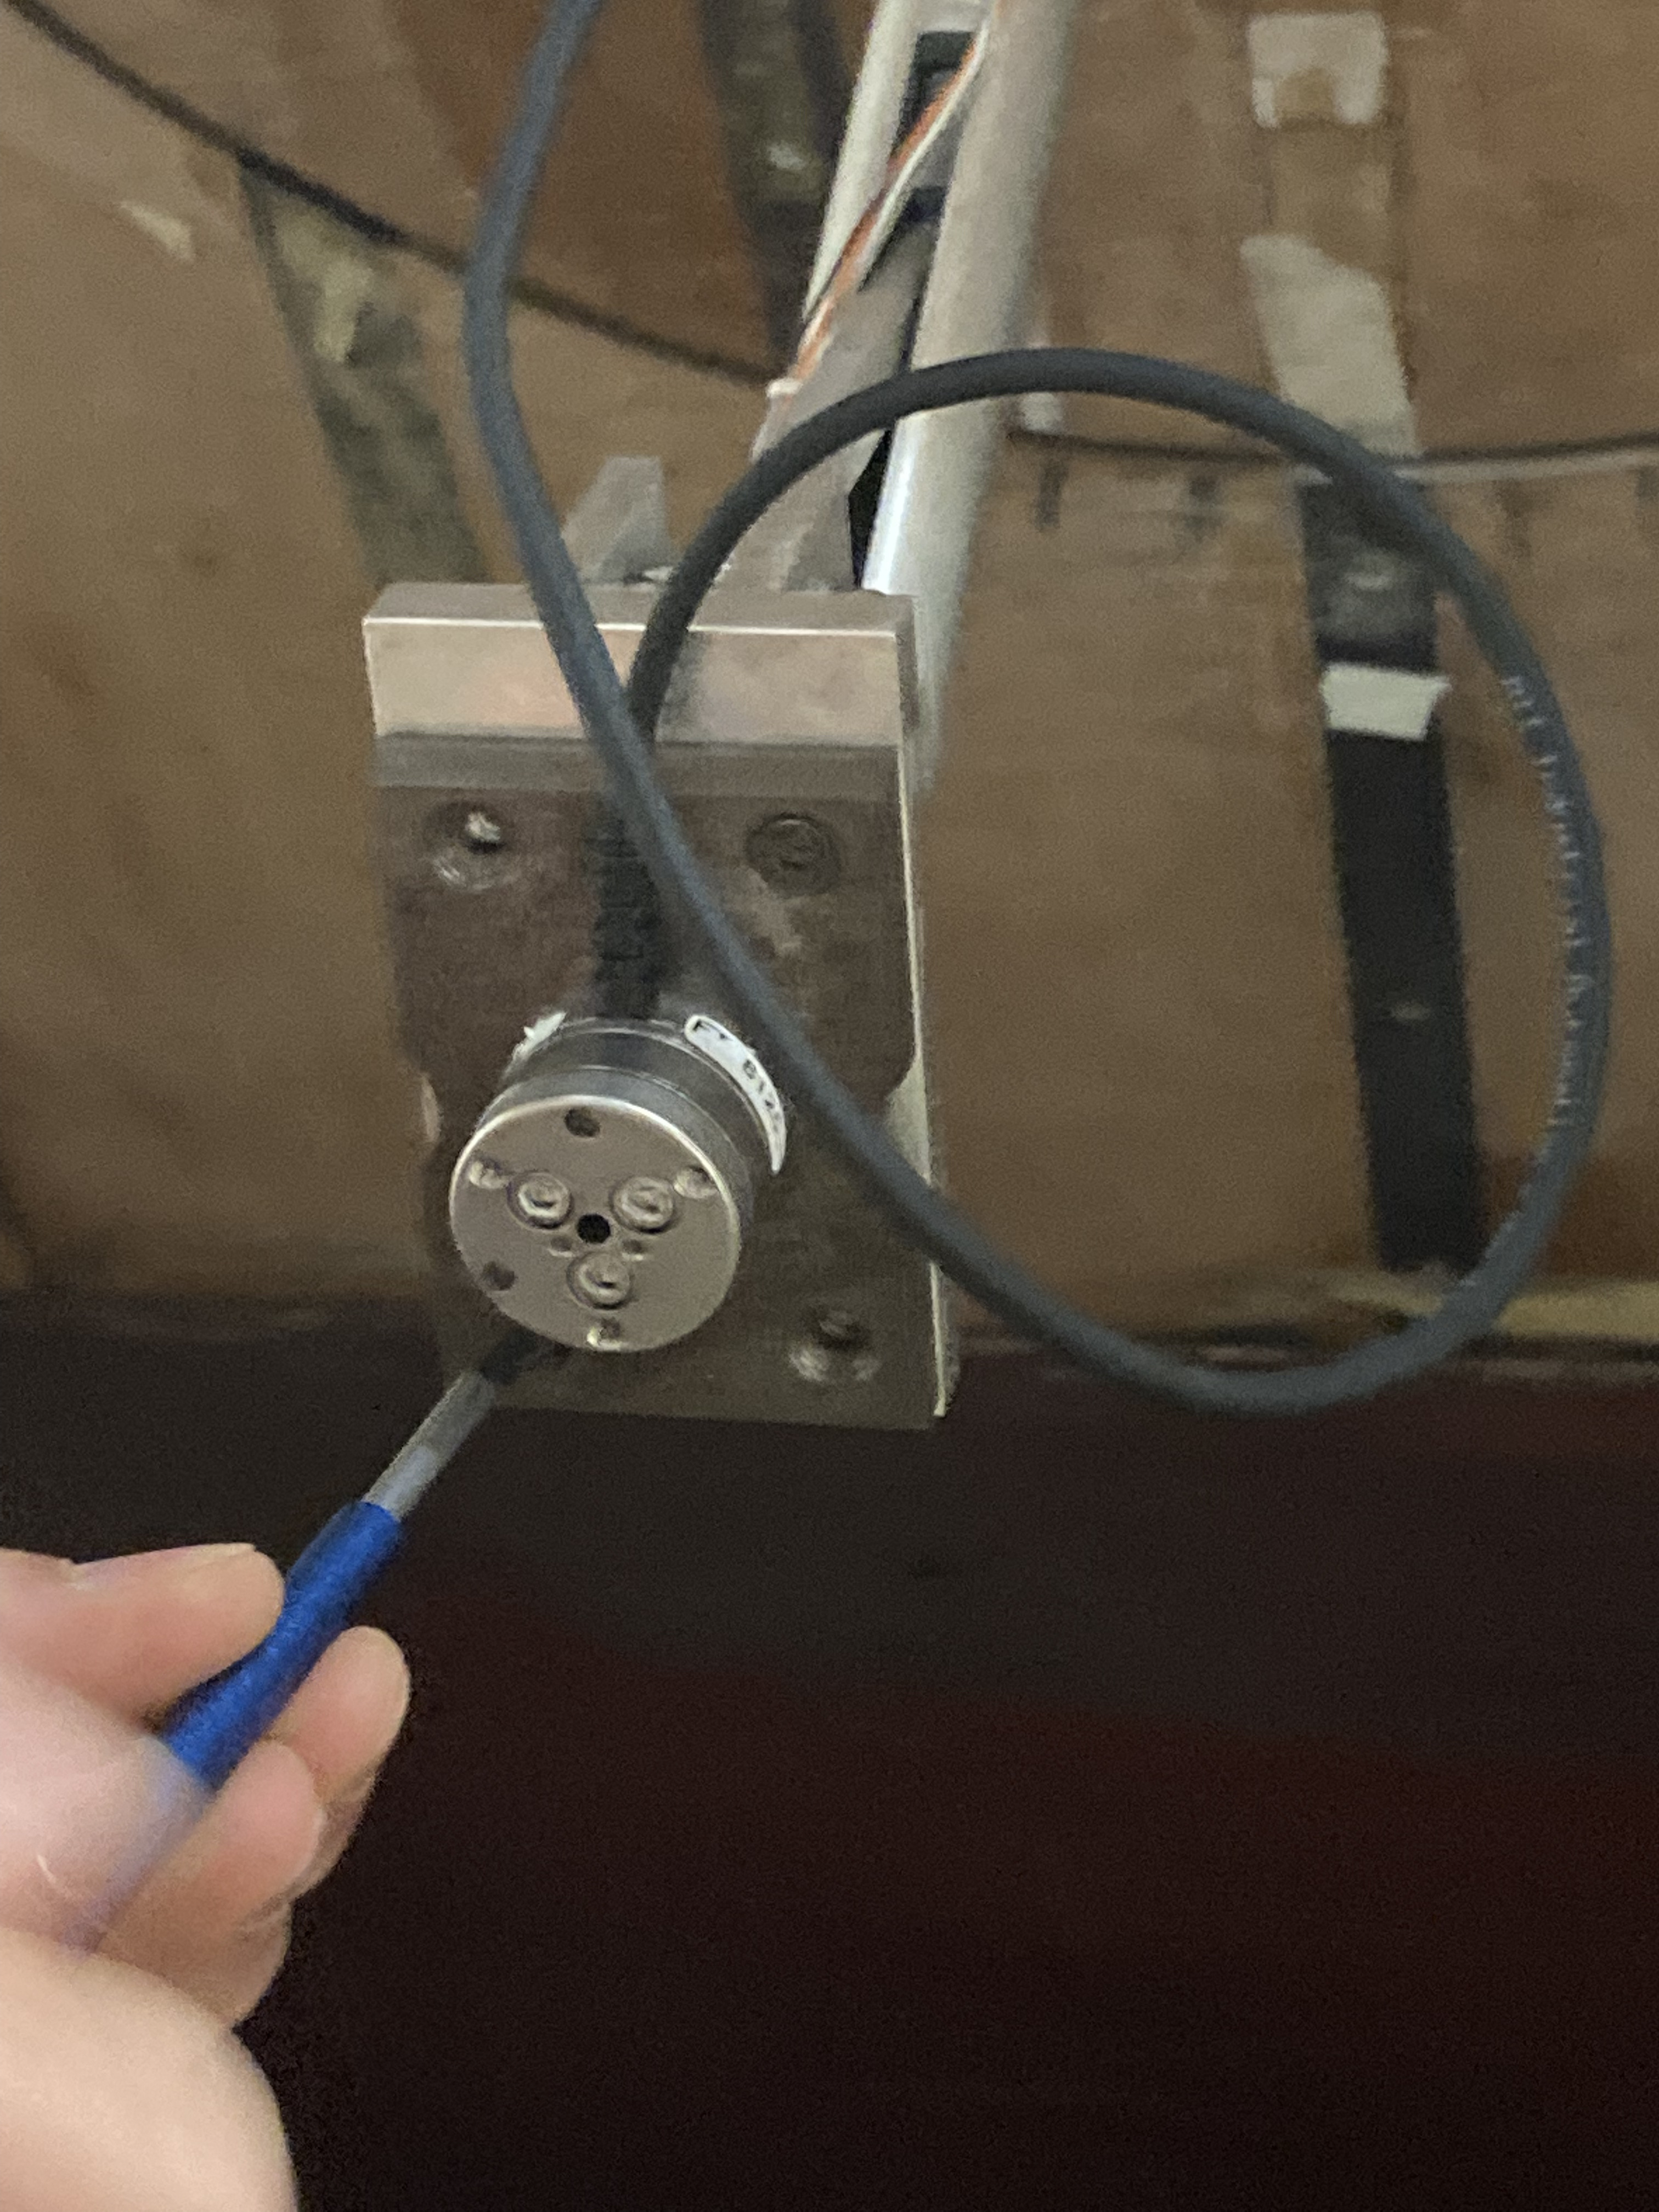
\includegraphics[scale=0.06]{04_Methodology/Figs/loadCellMount}
                \caption{Nano 25 load cell mount}
                \label{fig:LoadCella}
     \end{subfigure}
     \hfill
     \begin{subfigure}[b]{0.45\textwidth}
                 \centering
                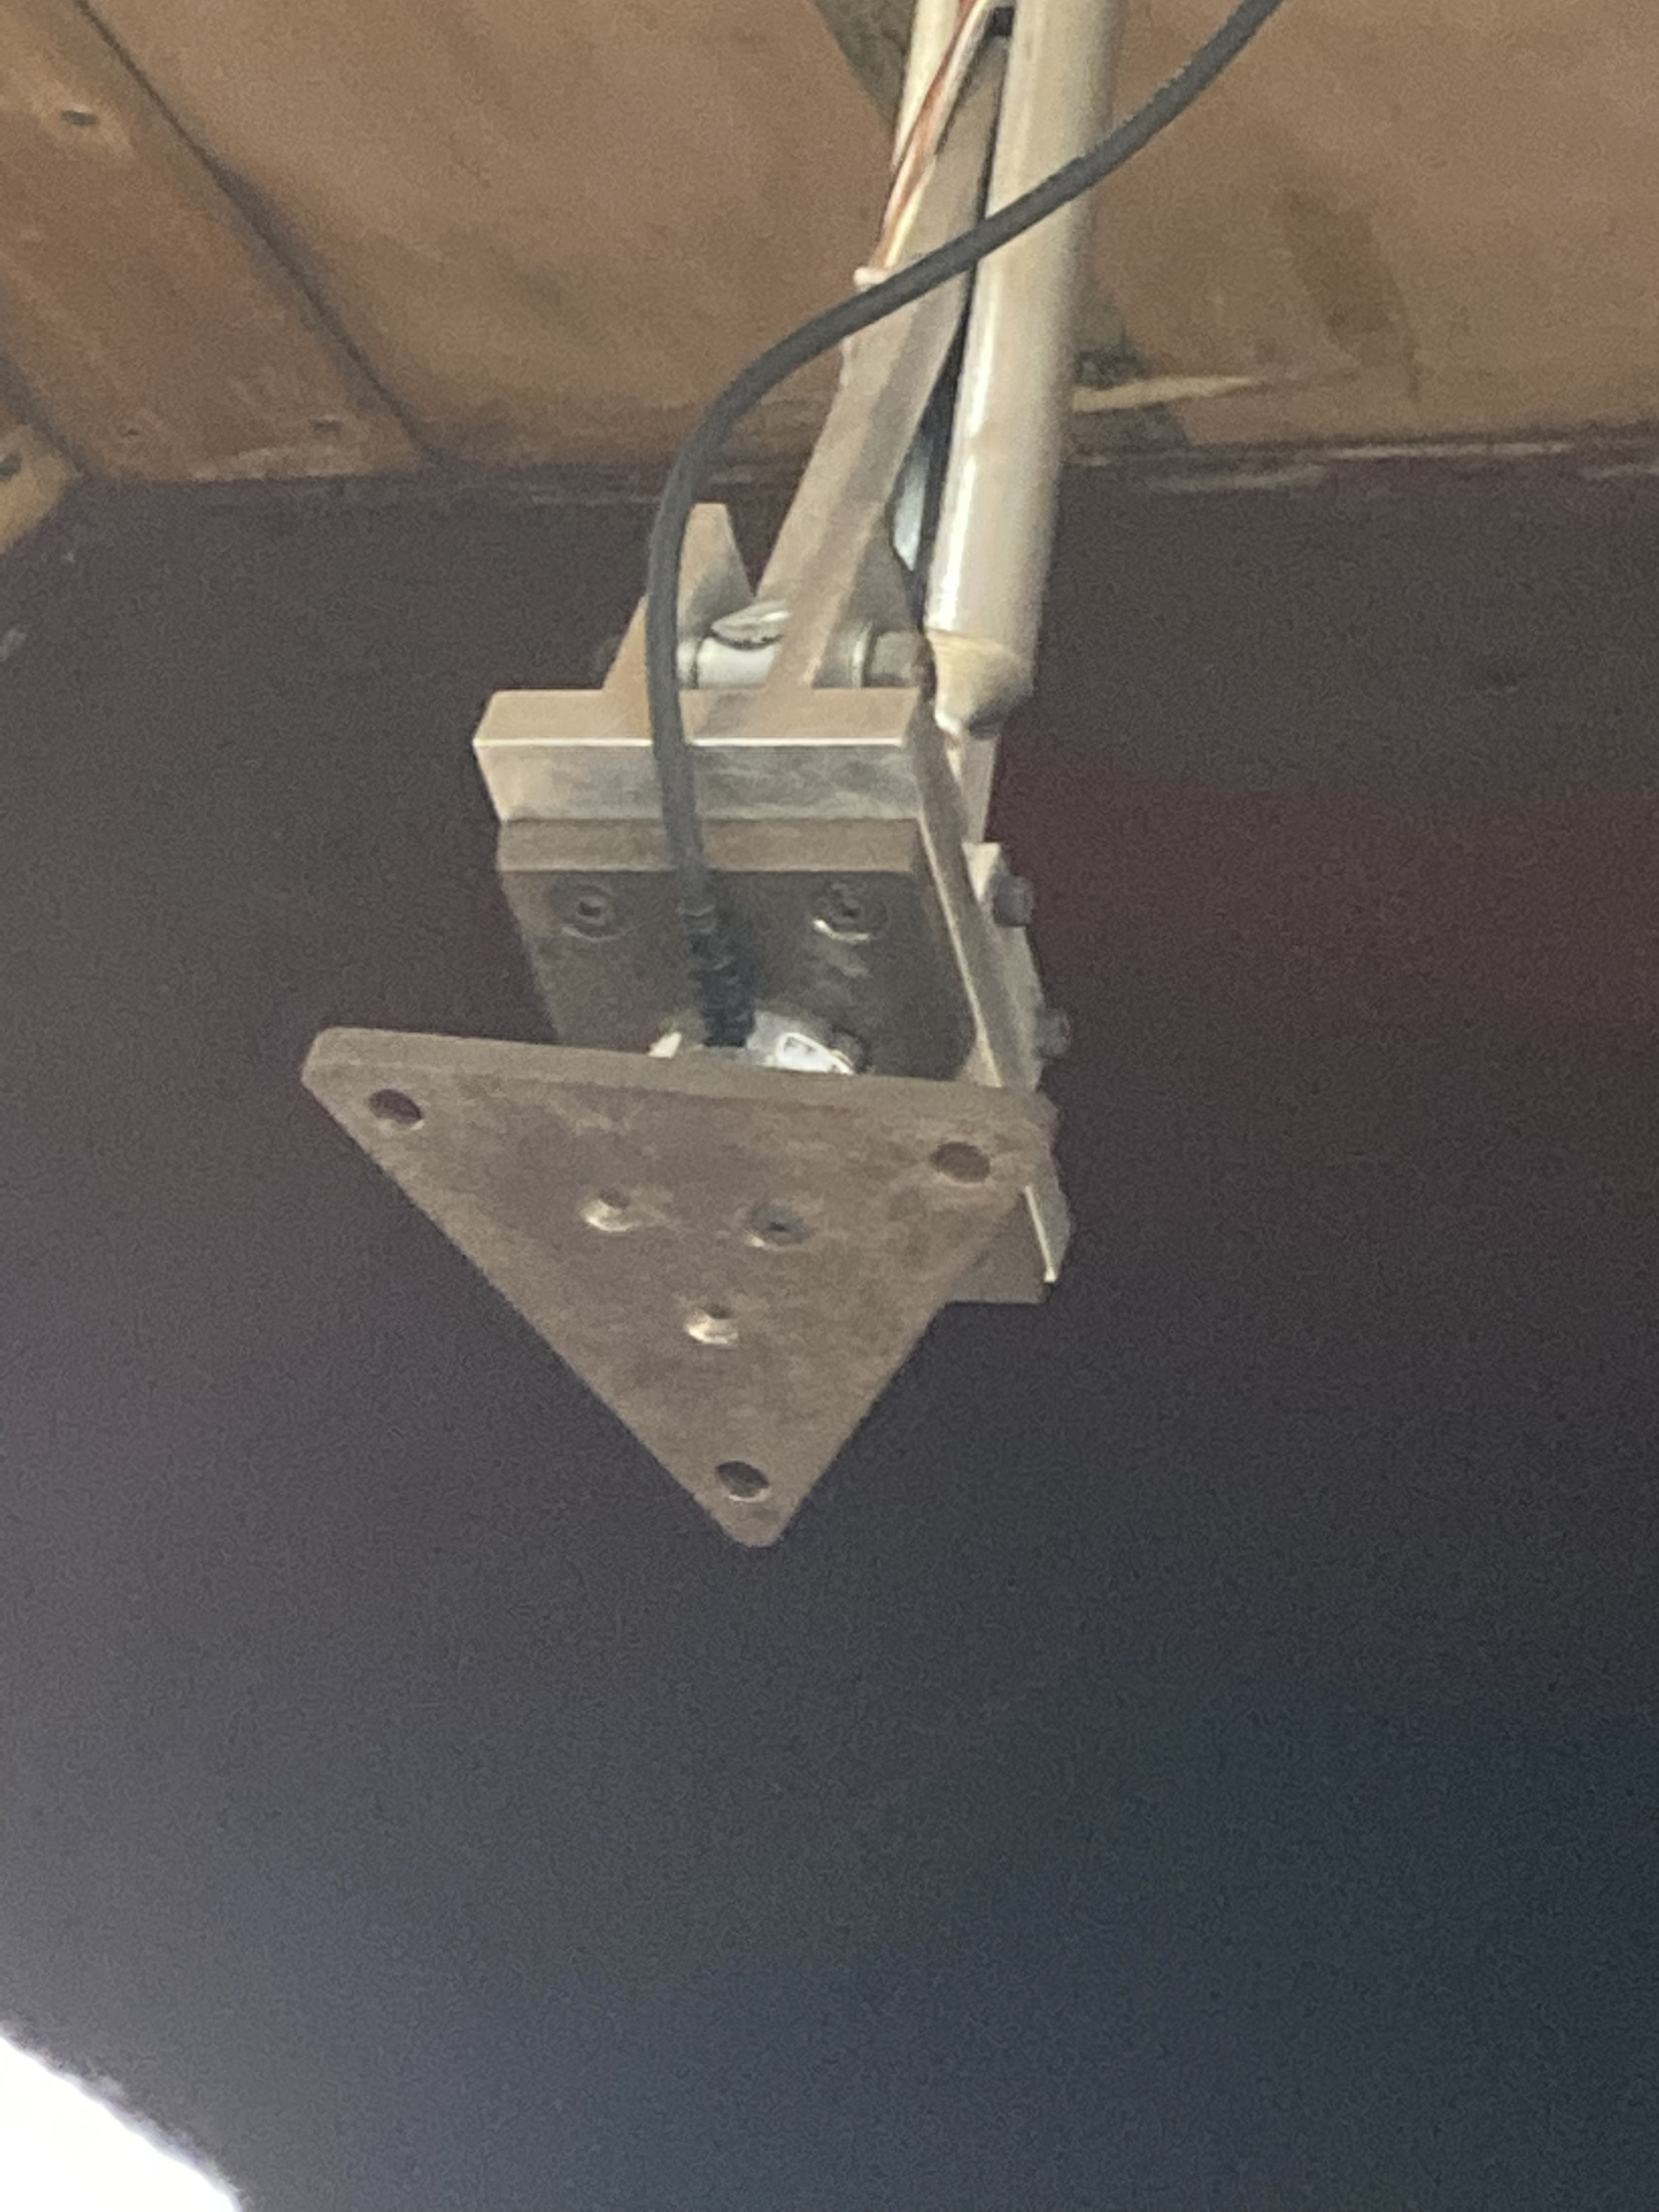
\includegraphics[scale=0.07]{04_Methodology/Figs/mount}
                \caption{Model mount in 3x4 wind tunnel}
                \label{fig:LoadCellb}
     \end{subfigure}
     \caption{Wind tunnel mount and load cell used}
     \label{fig:loadMount}

\end{figure}


% \begin{figure}[H]
%     \centering
%     \begin{subfigure}[b]{0.3\textwidth}
%         \centering
%         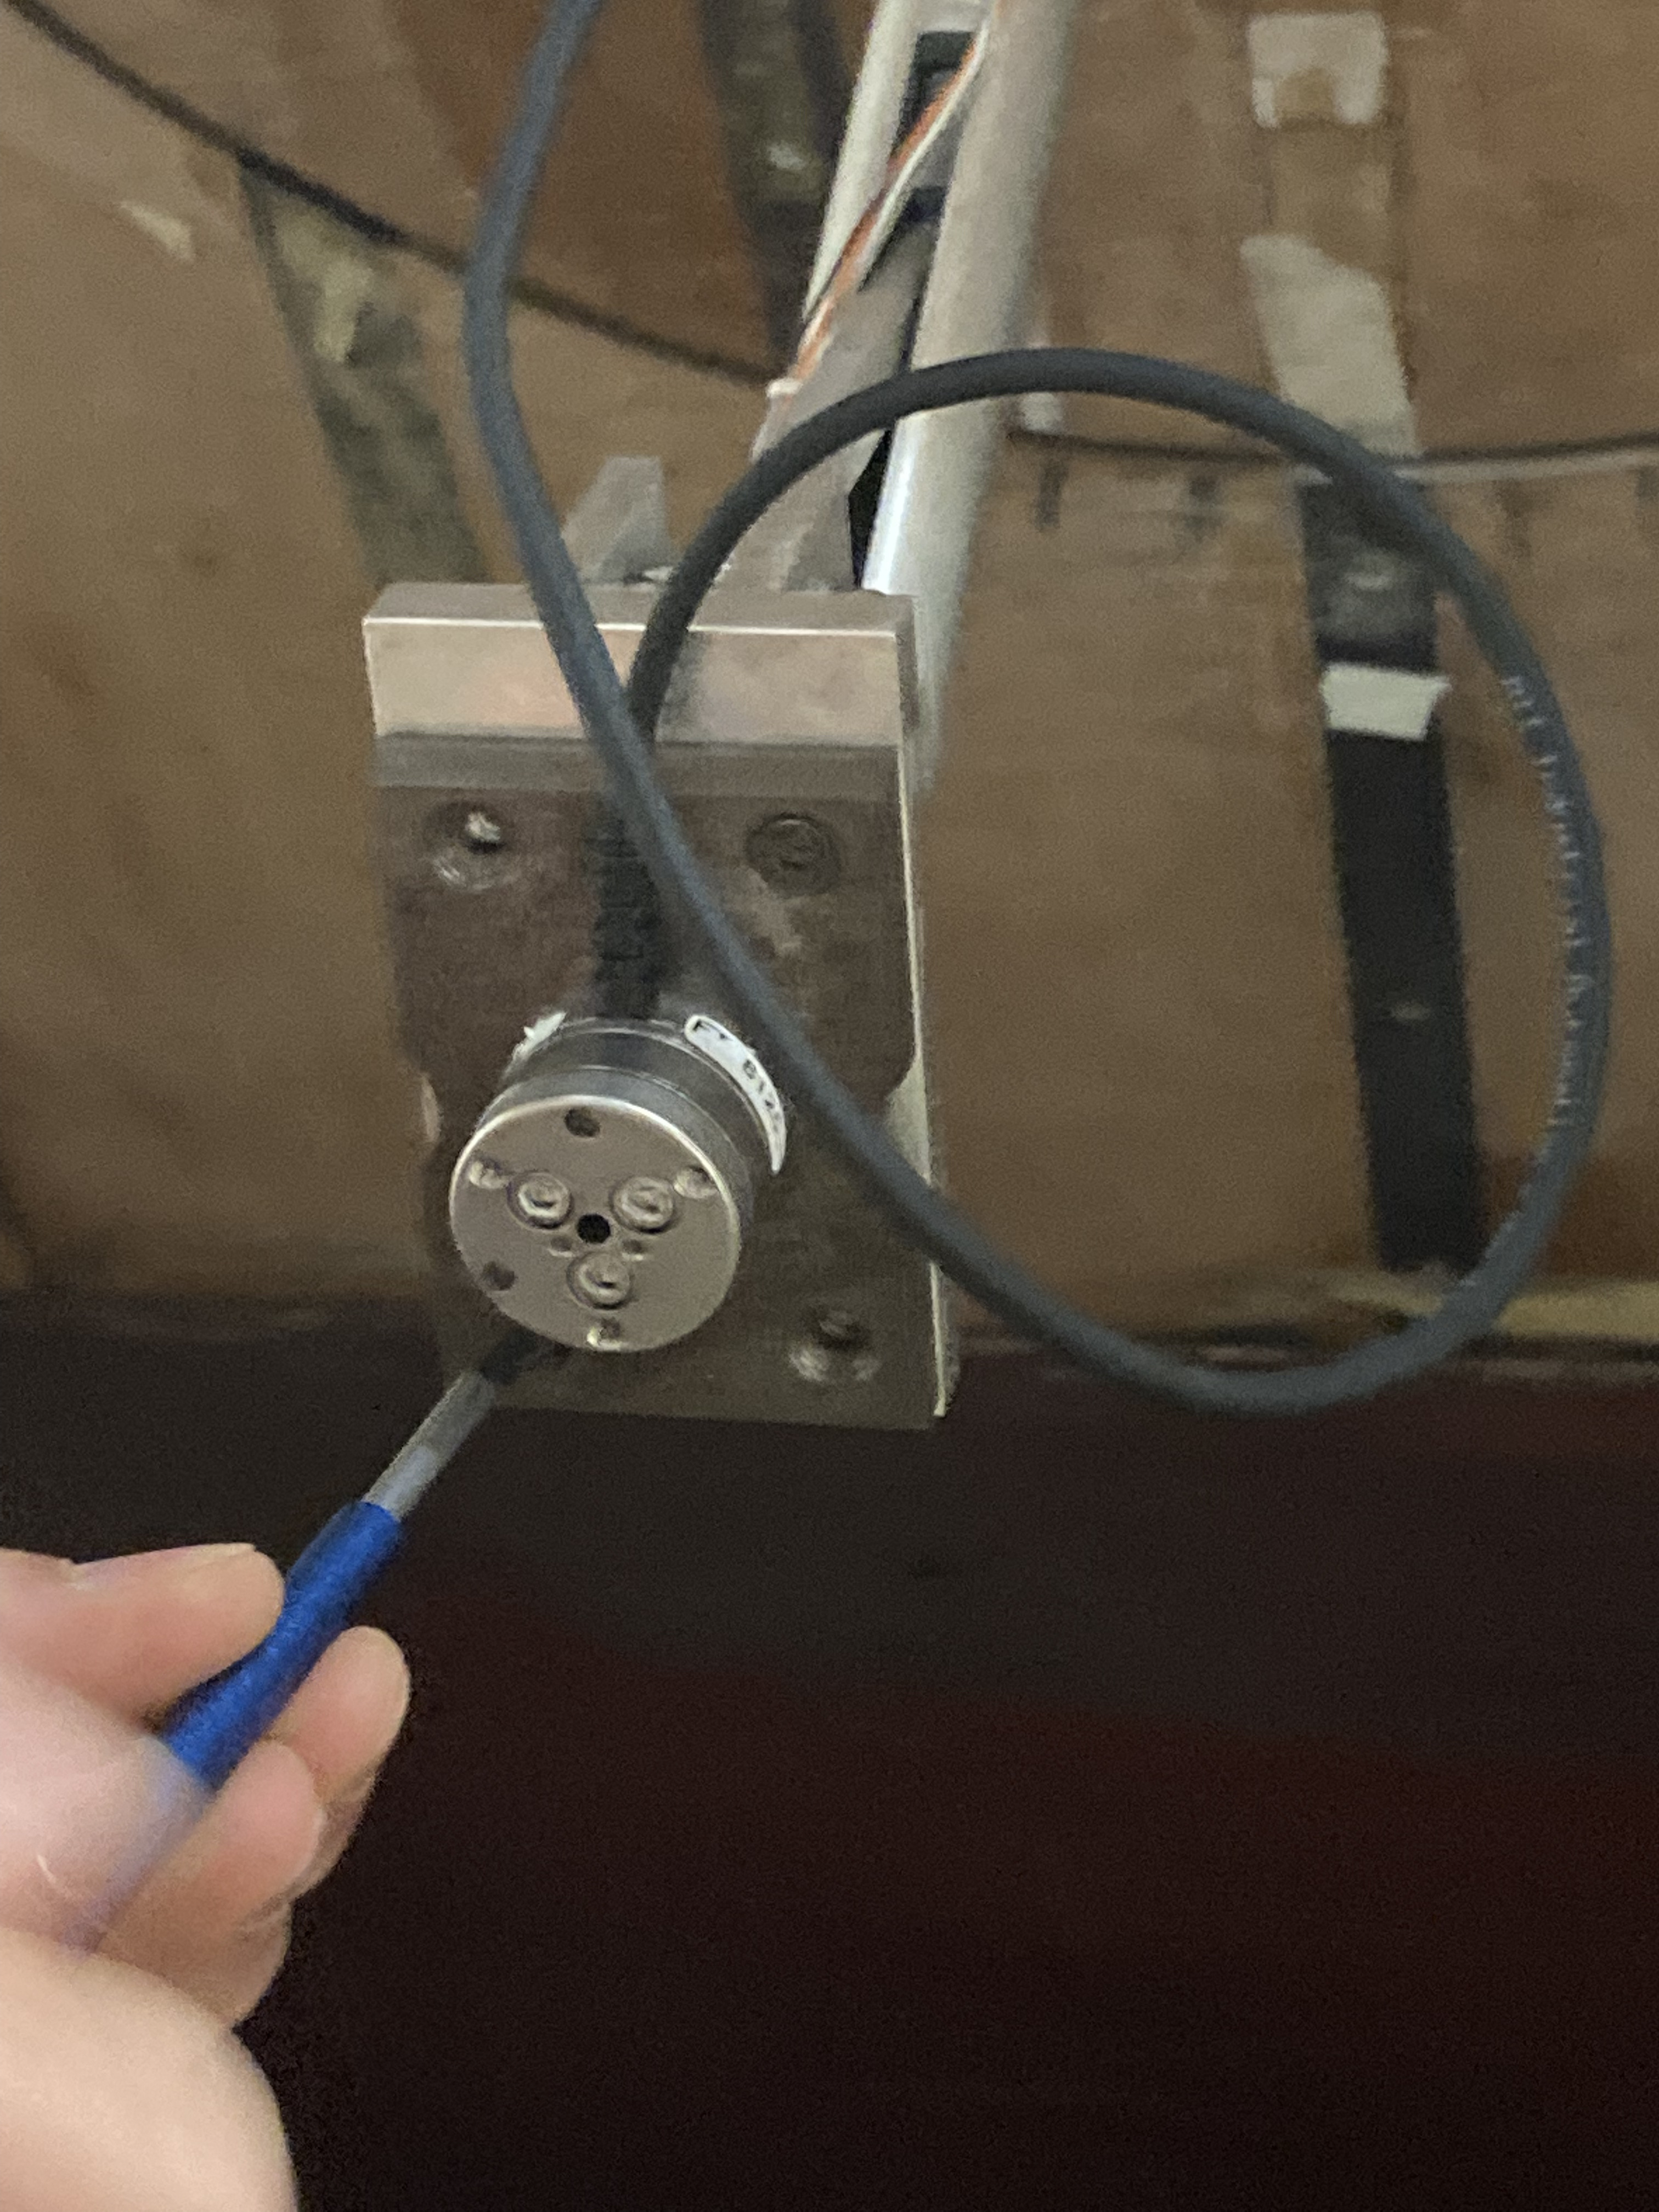
\includegraphics[scale=0.08]{04_Methodology/Figs/loadCellMount}
%         \caption{Nano 25 load cell mount}
%         \label{fig:LoadCella}
%     \end{subfigure}

%     \hfill
%     \begin{subfigure}[b]{0.3\textwidth}
%         \centering
%         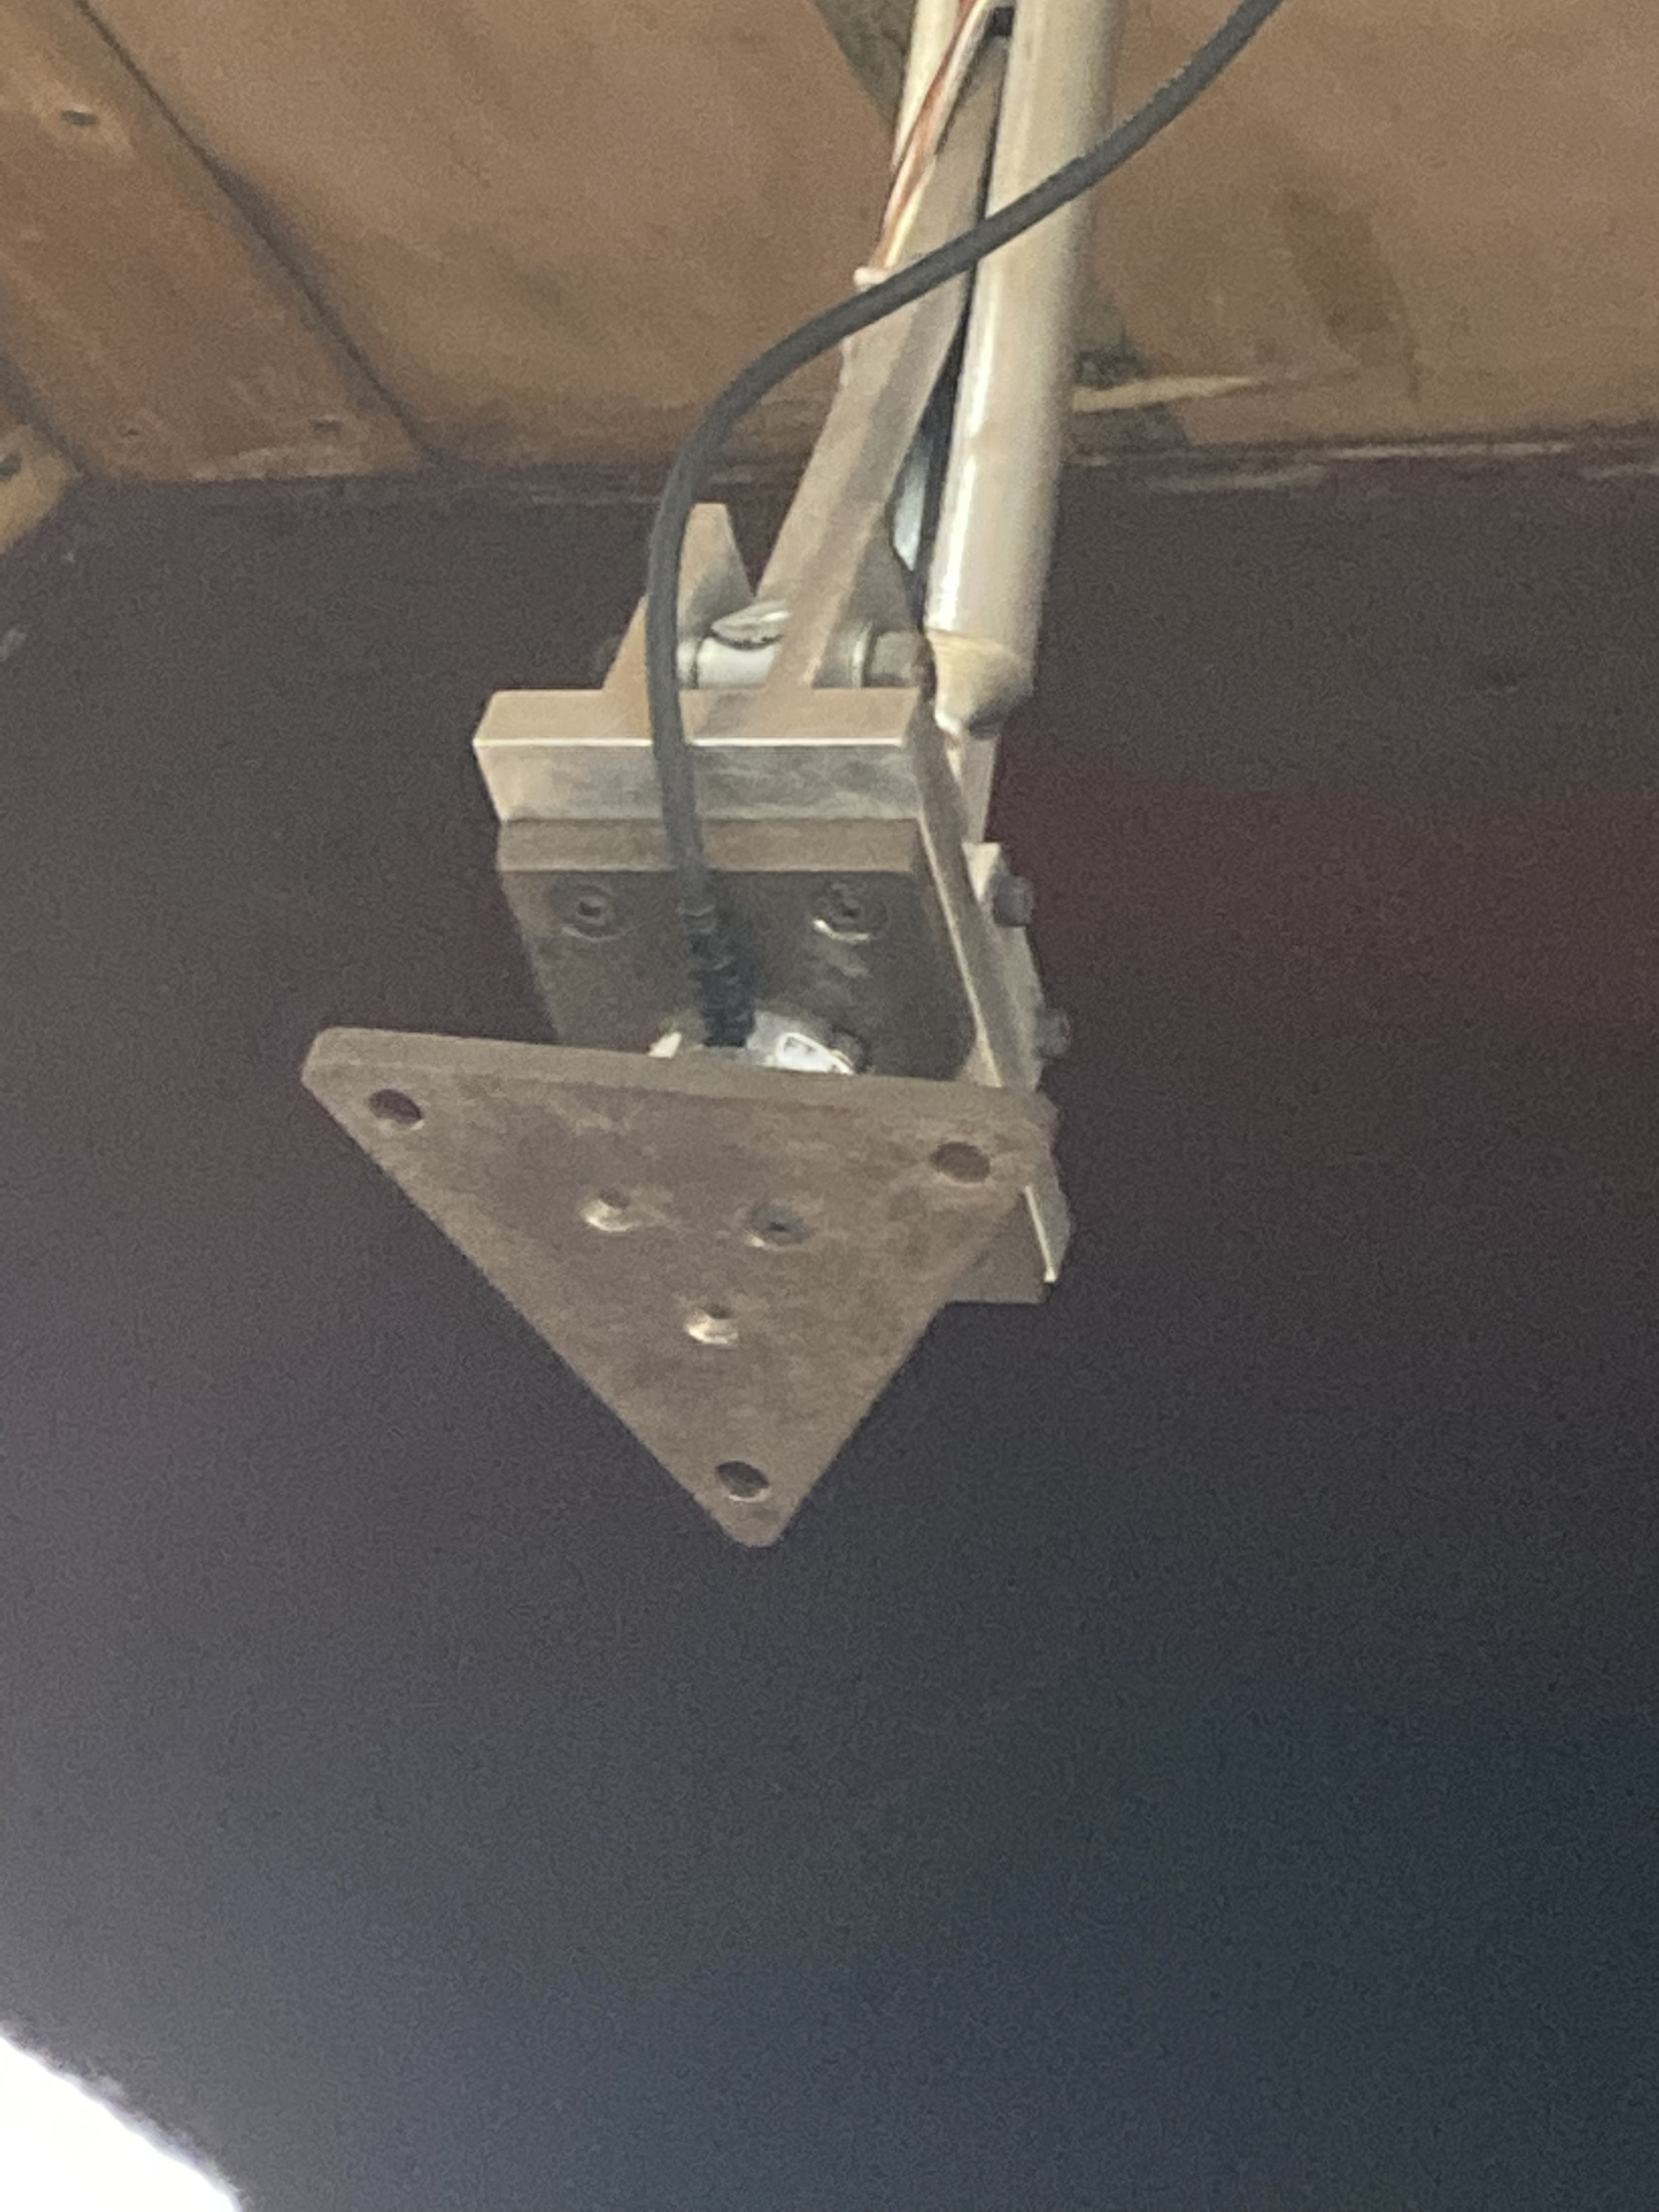
\includegraphics[scale=0.1]{04_Methodology/Figs/mount}
%         \caption{Model mount in 3x4 wind tunnel}
%         \label{fig:LoadCellb}
%     \end{subfigure}
%     \hfill
    
% \end{figure}


The model was then attached in three main configurations. These were mounting the propeller without a propeller, in a pusher and tractor configurations. These configurations are shown from Figure \Cref{fig:noprop} to Figure \Cref{fig:tractors} respectively.


\begin{figure}[H]
     \centering
     \begin{subfigure}[b]{0.3\textwidth}
         \centering
         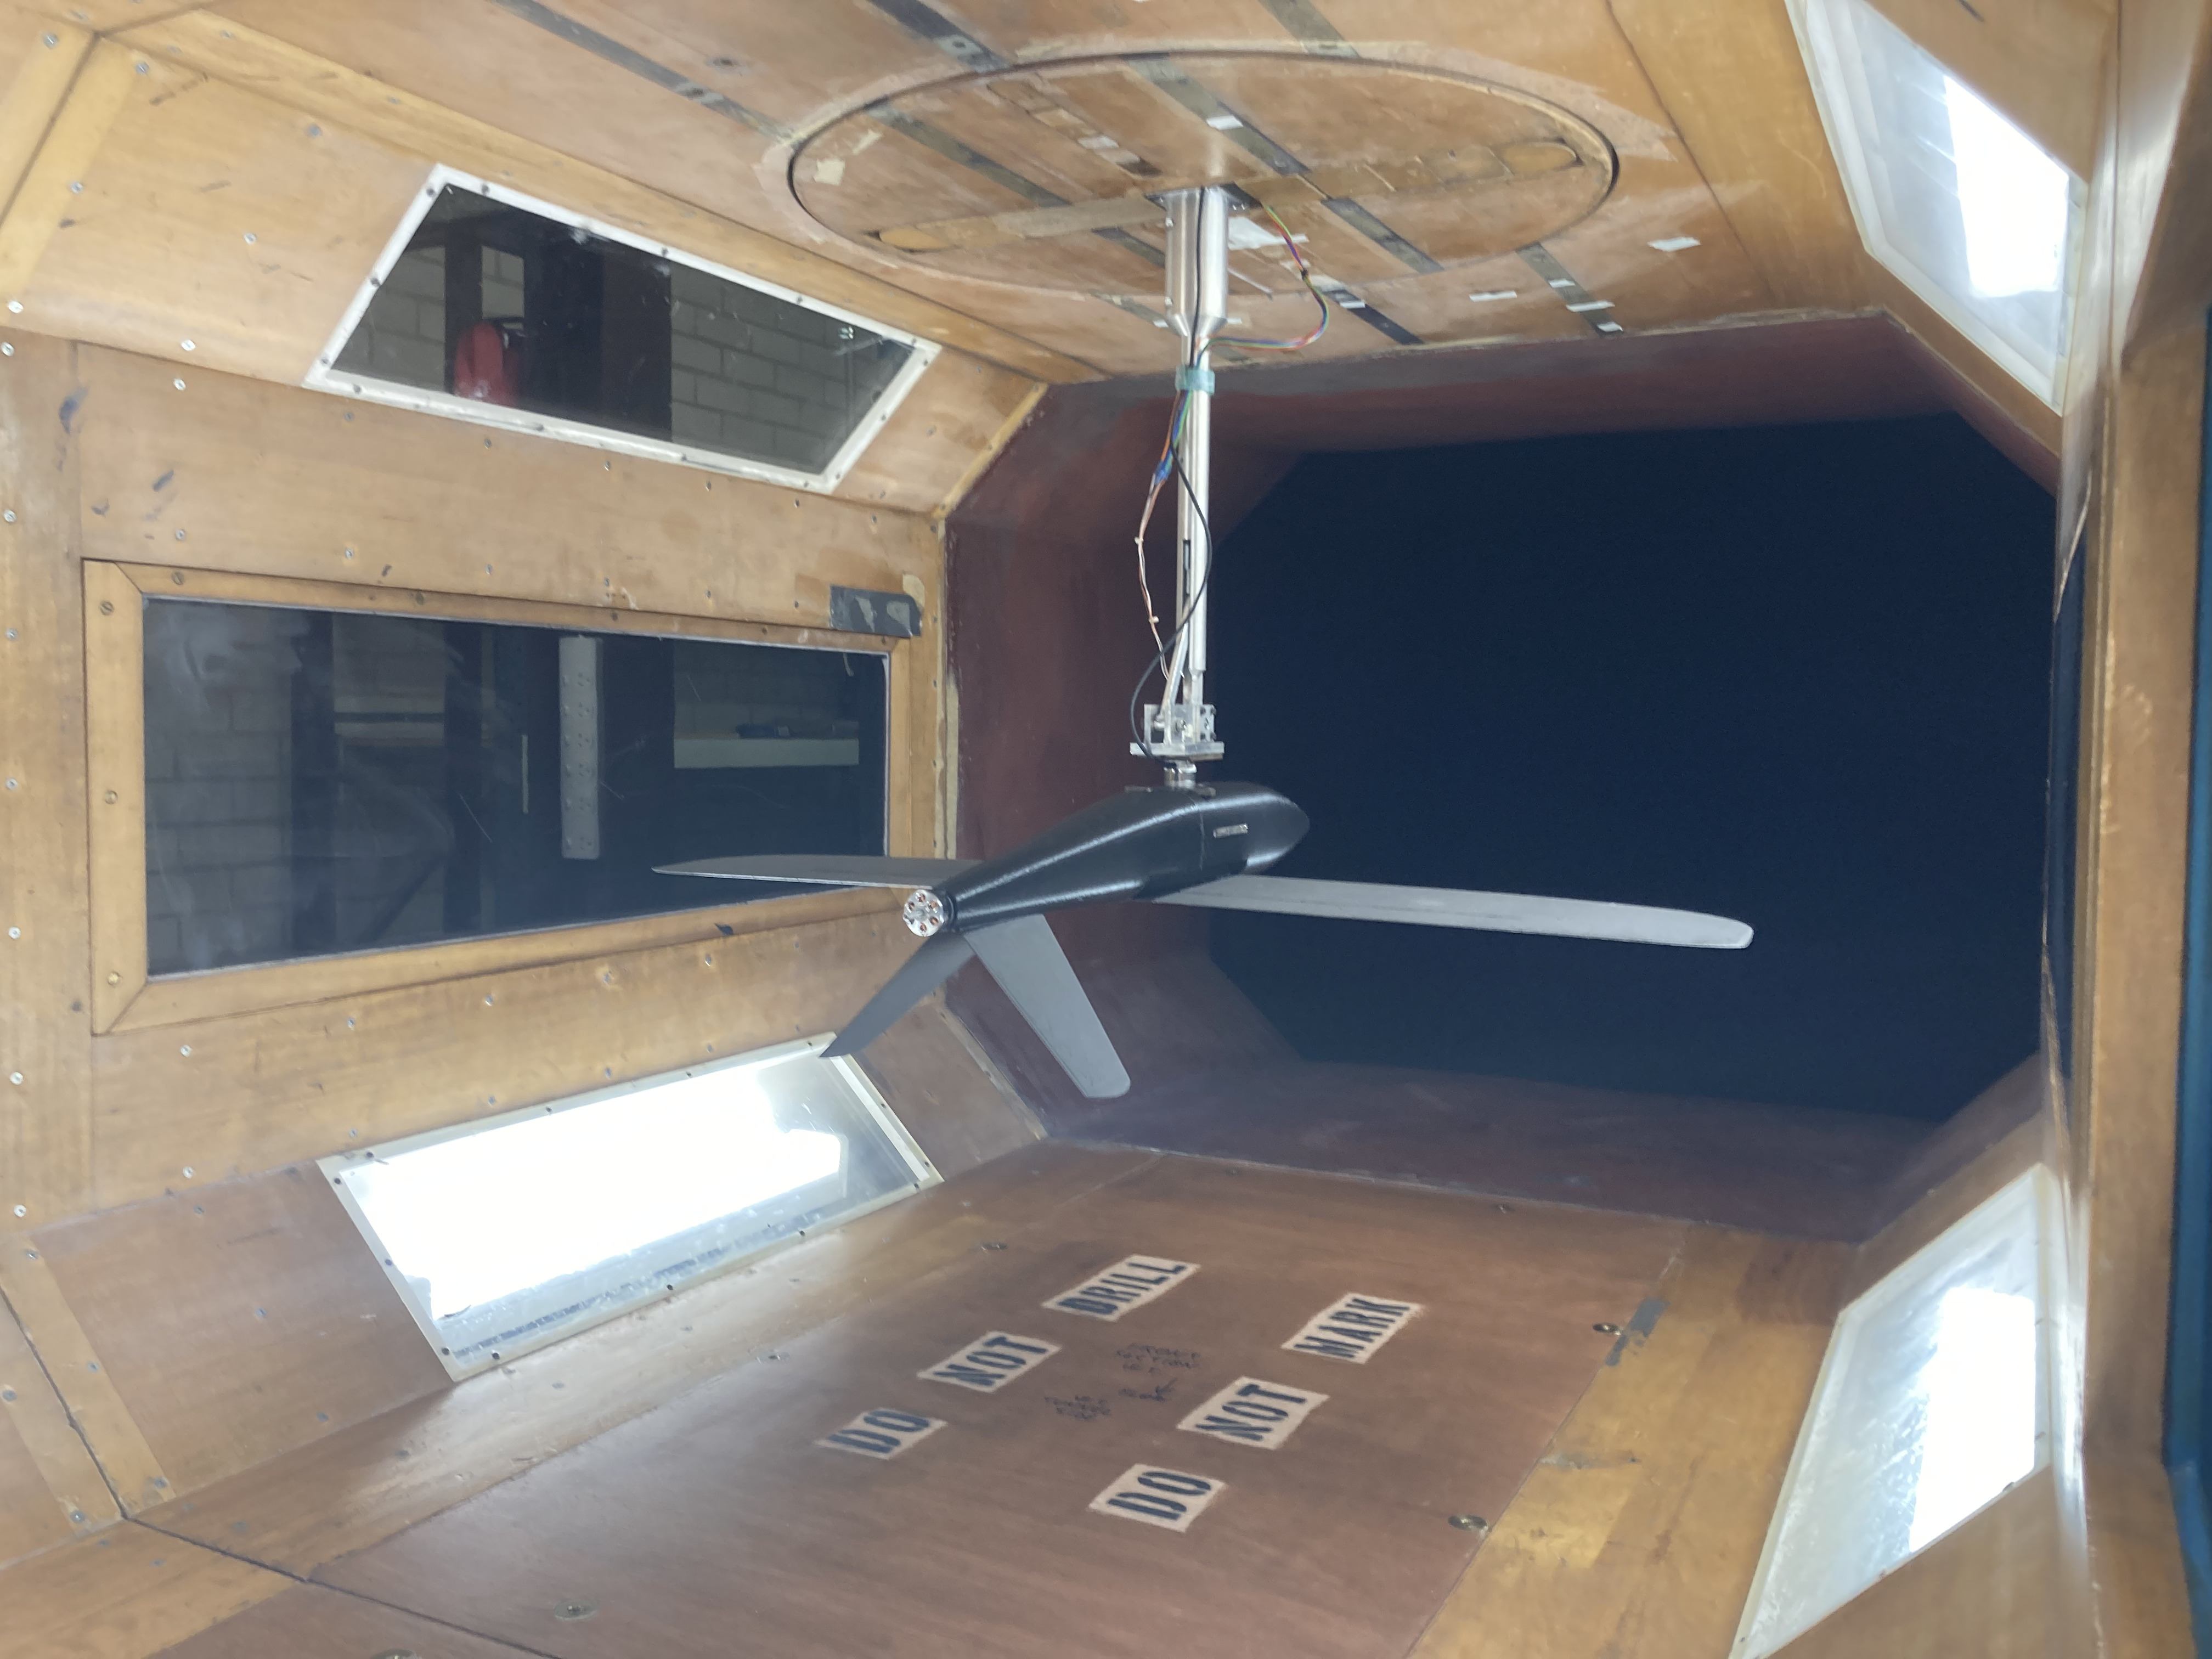
\includegraphics[scale=0.03]{04_Methodology/Figs/noprop}
         \caption{Model with no propeller attached}
          \label{fig:noprop}
     \end{subfigure}
     \hfill
     \begin{subfigure}[b]{0.3\textwidth}
             \centering
             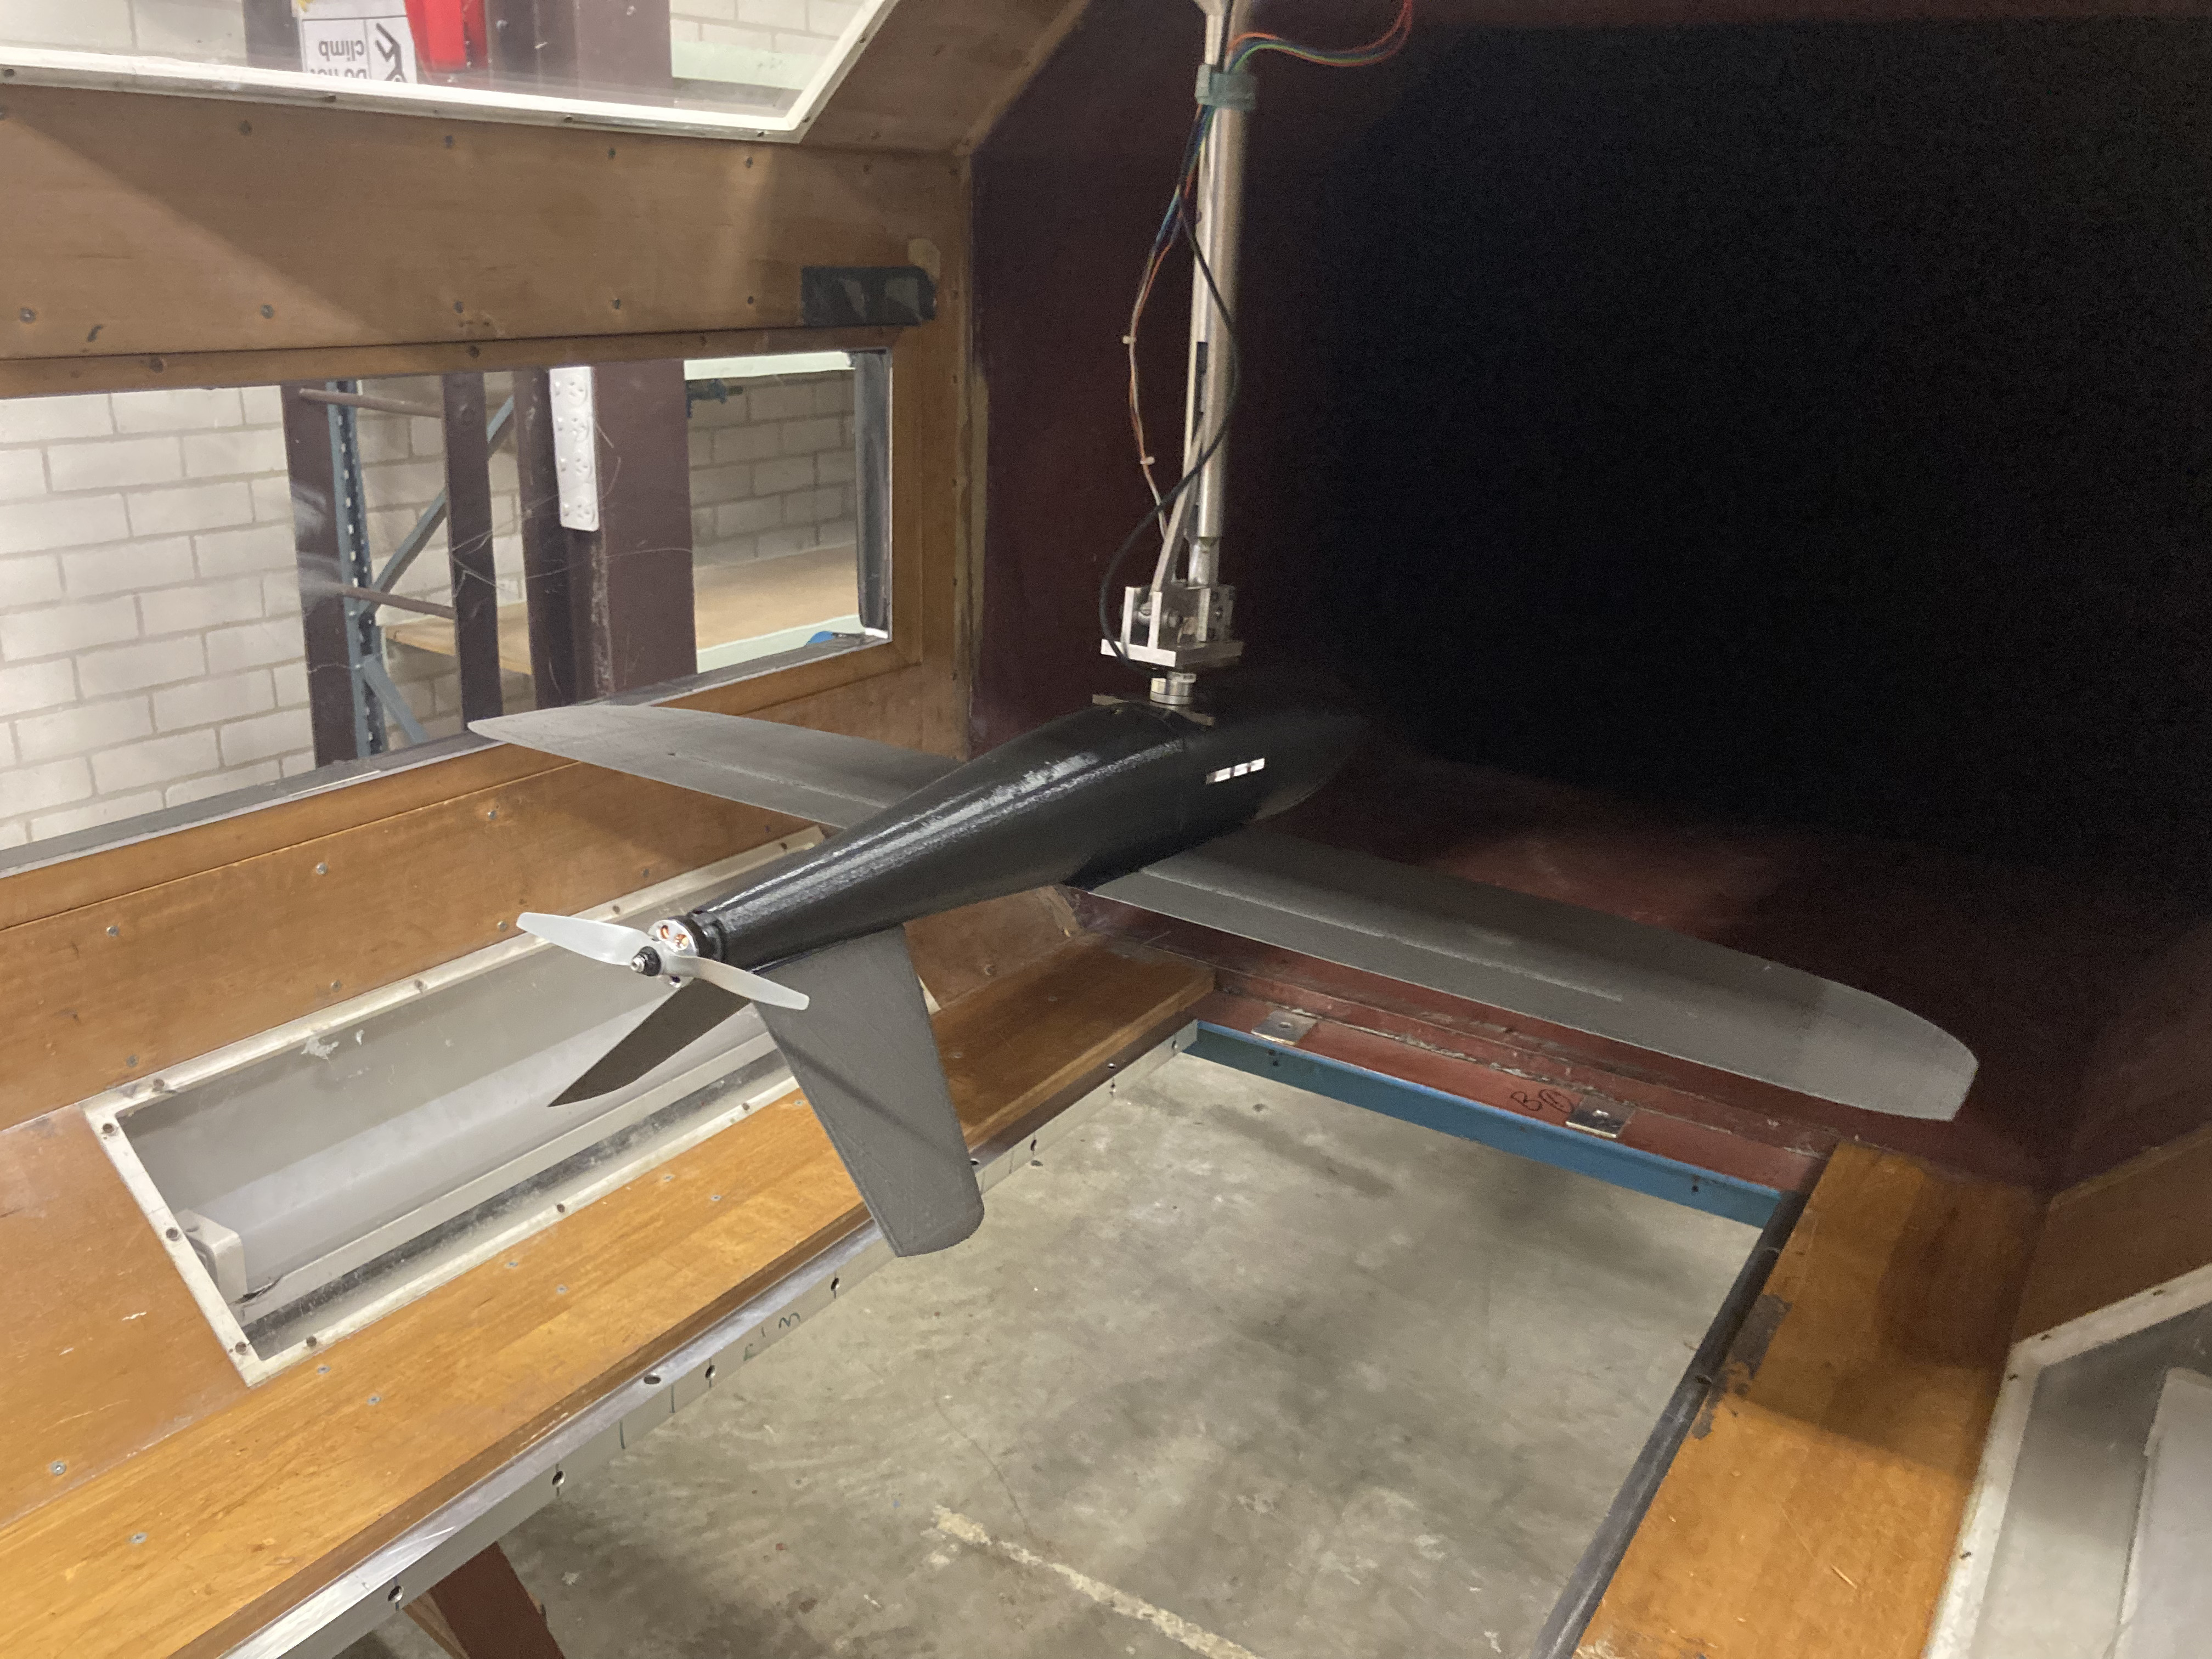
\includegraphics[scale = 0.03]{04_Methodology/Figs/pusher}
             \caption{Model in pusher configuration}
             \label{fig:pusher}
     \end{subfigure}
     \hfill
     \begin{subfigure}[b]{0.3\textwidth}
             \centering
             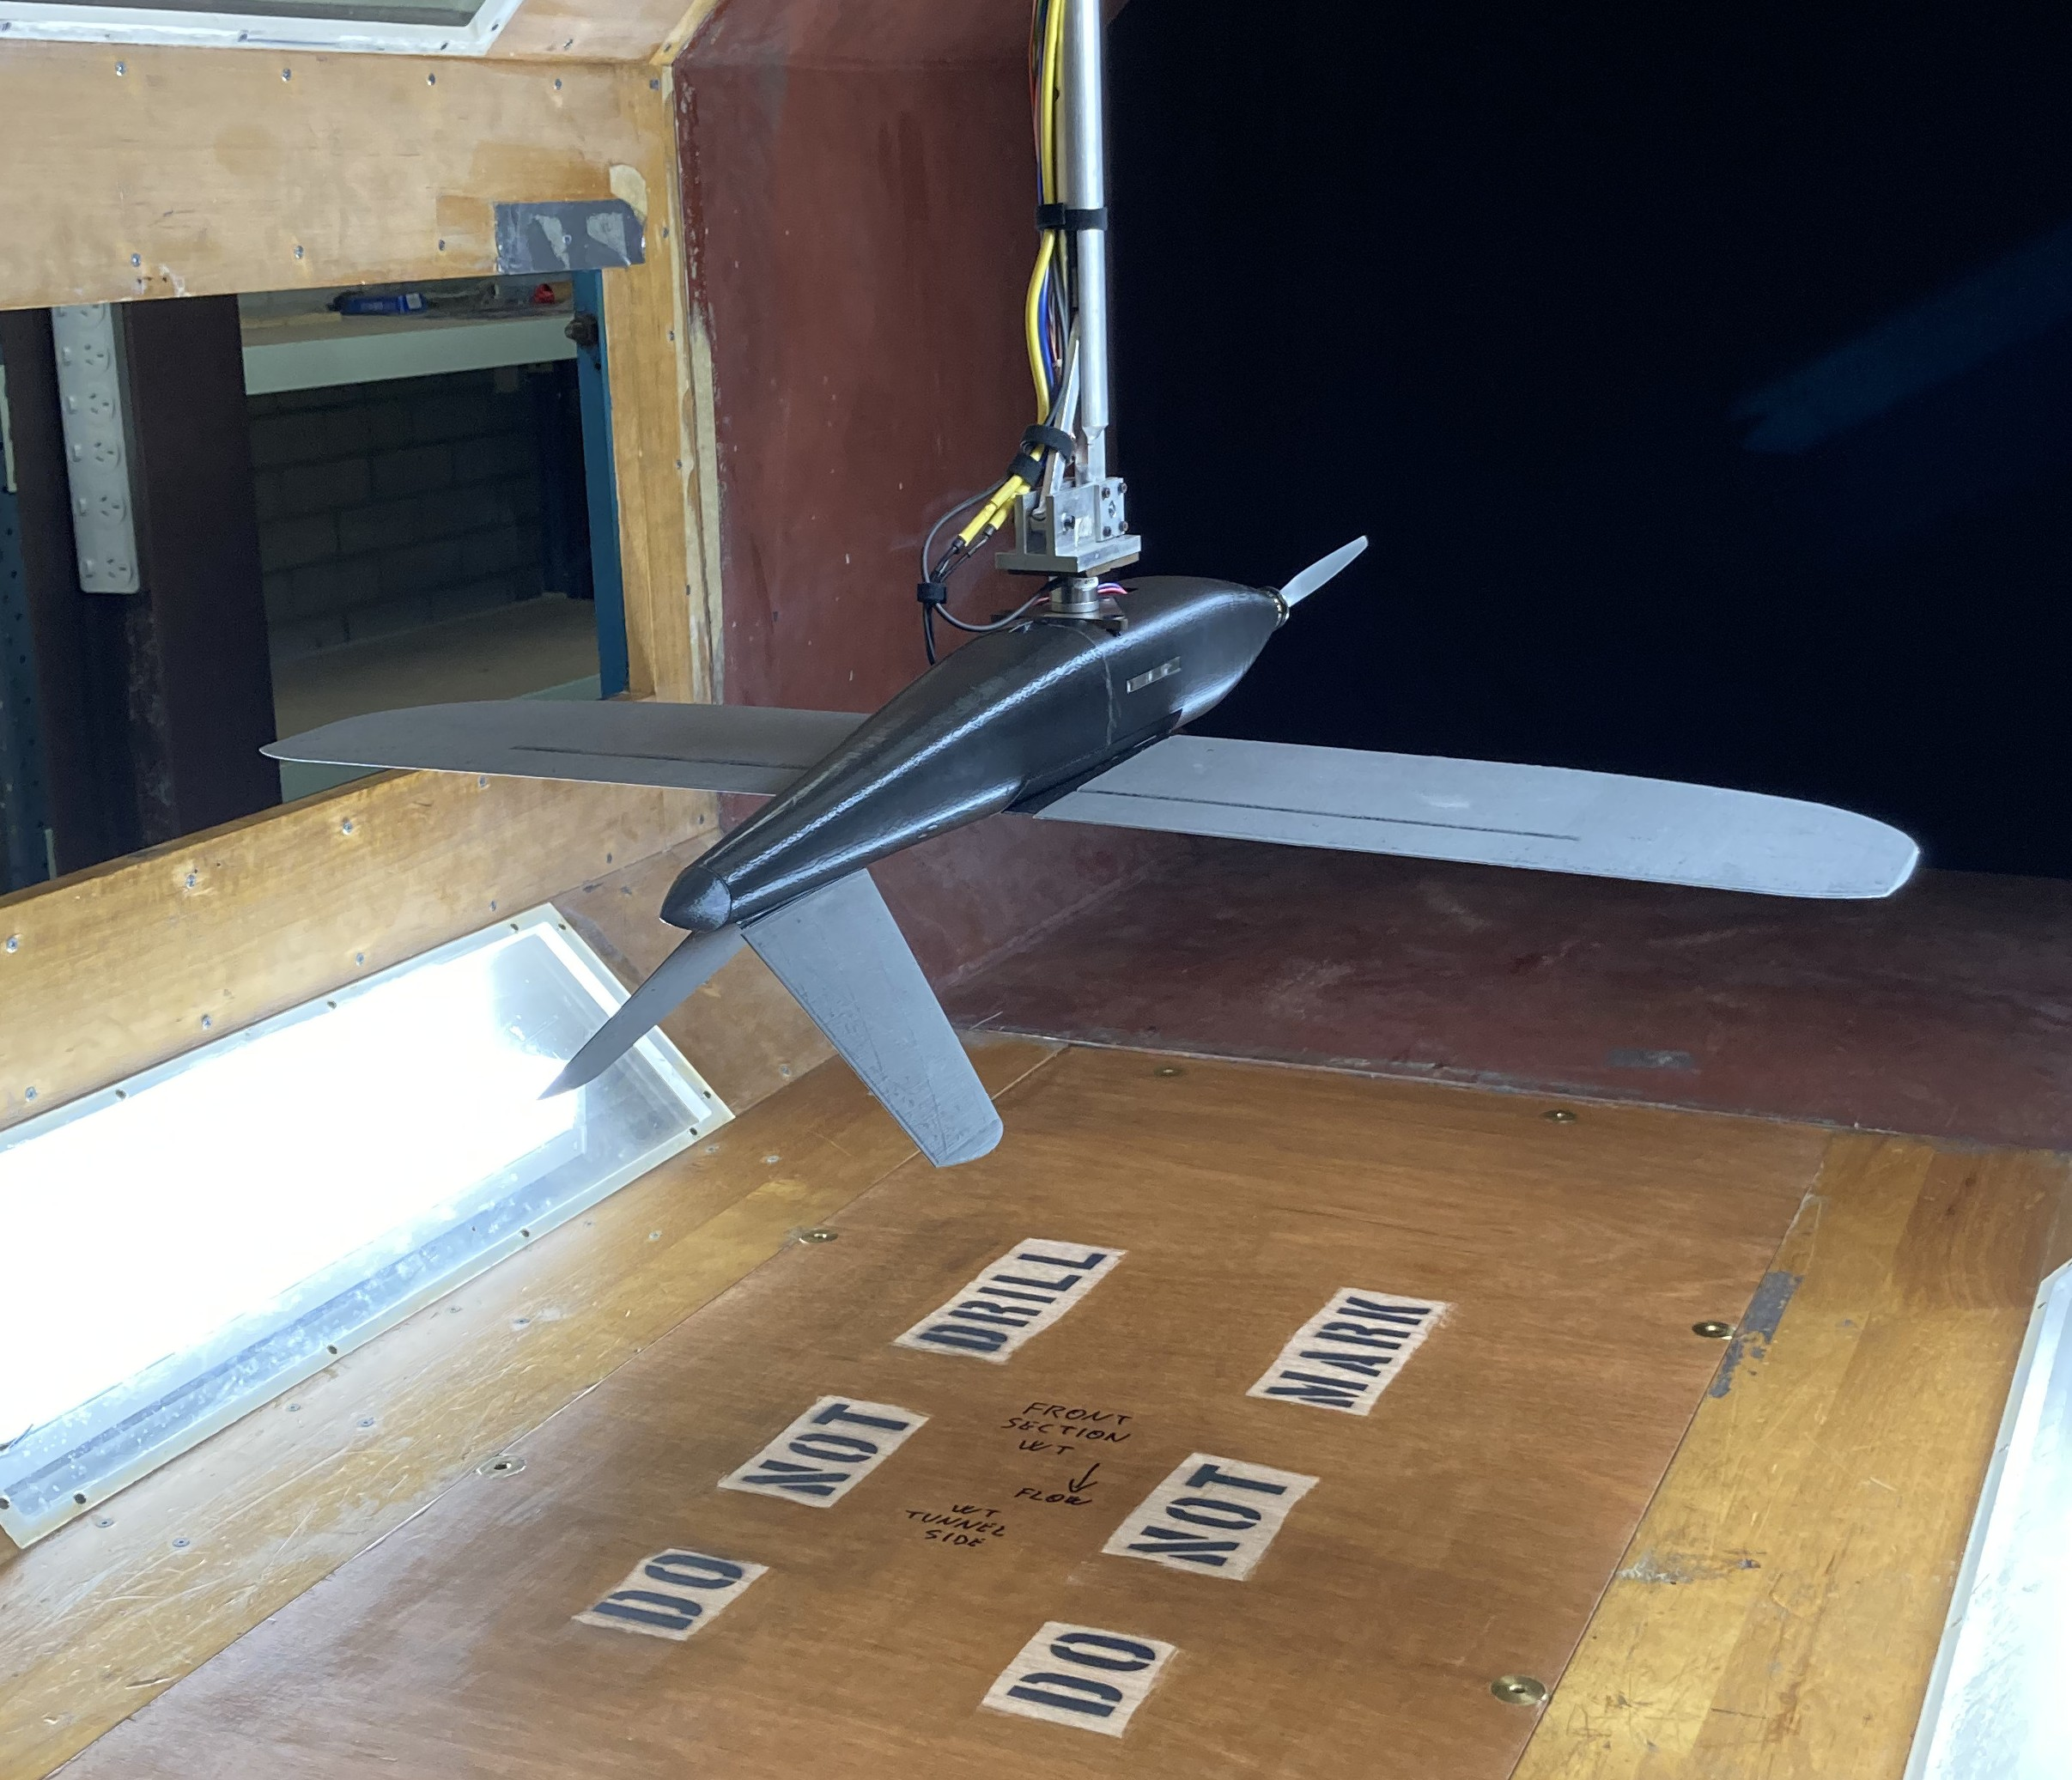
\includegraphics[scale=0.05]{04_Methodology/Figs/tractors}
             \caption{Model in tractor configuration}
             \label{fig:tractors}
     \end{subfigure}
        \caption{Examples of MAVs with category}
        \label{fig:typesUsed}
\end{figure}


The wind tunnel was then calibrated for wind speed, atmospheric conditions and angles of attack. The mount used for the model was double-checked using a pitch gauge to ensure the angle of attack was correct as shown in Figure \ref{fig:pitchGauge}. 


\begin{figure}[H]
    \centering
    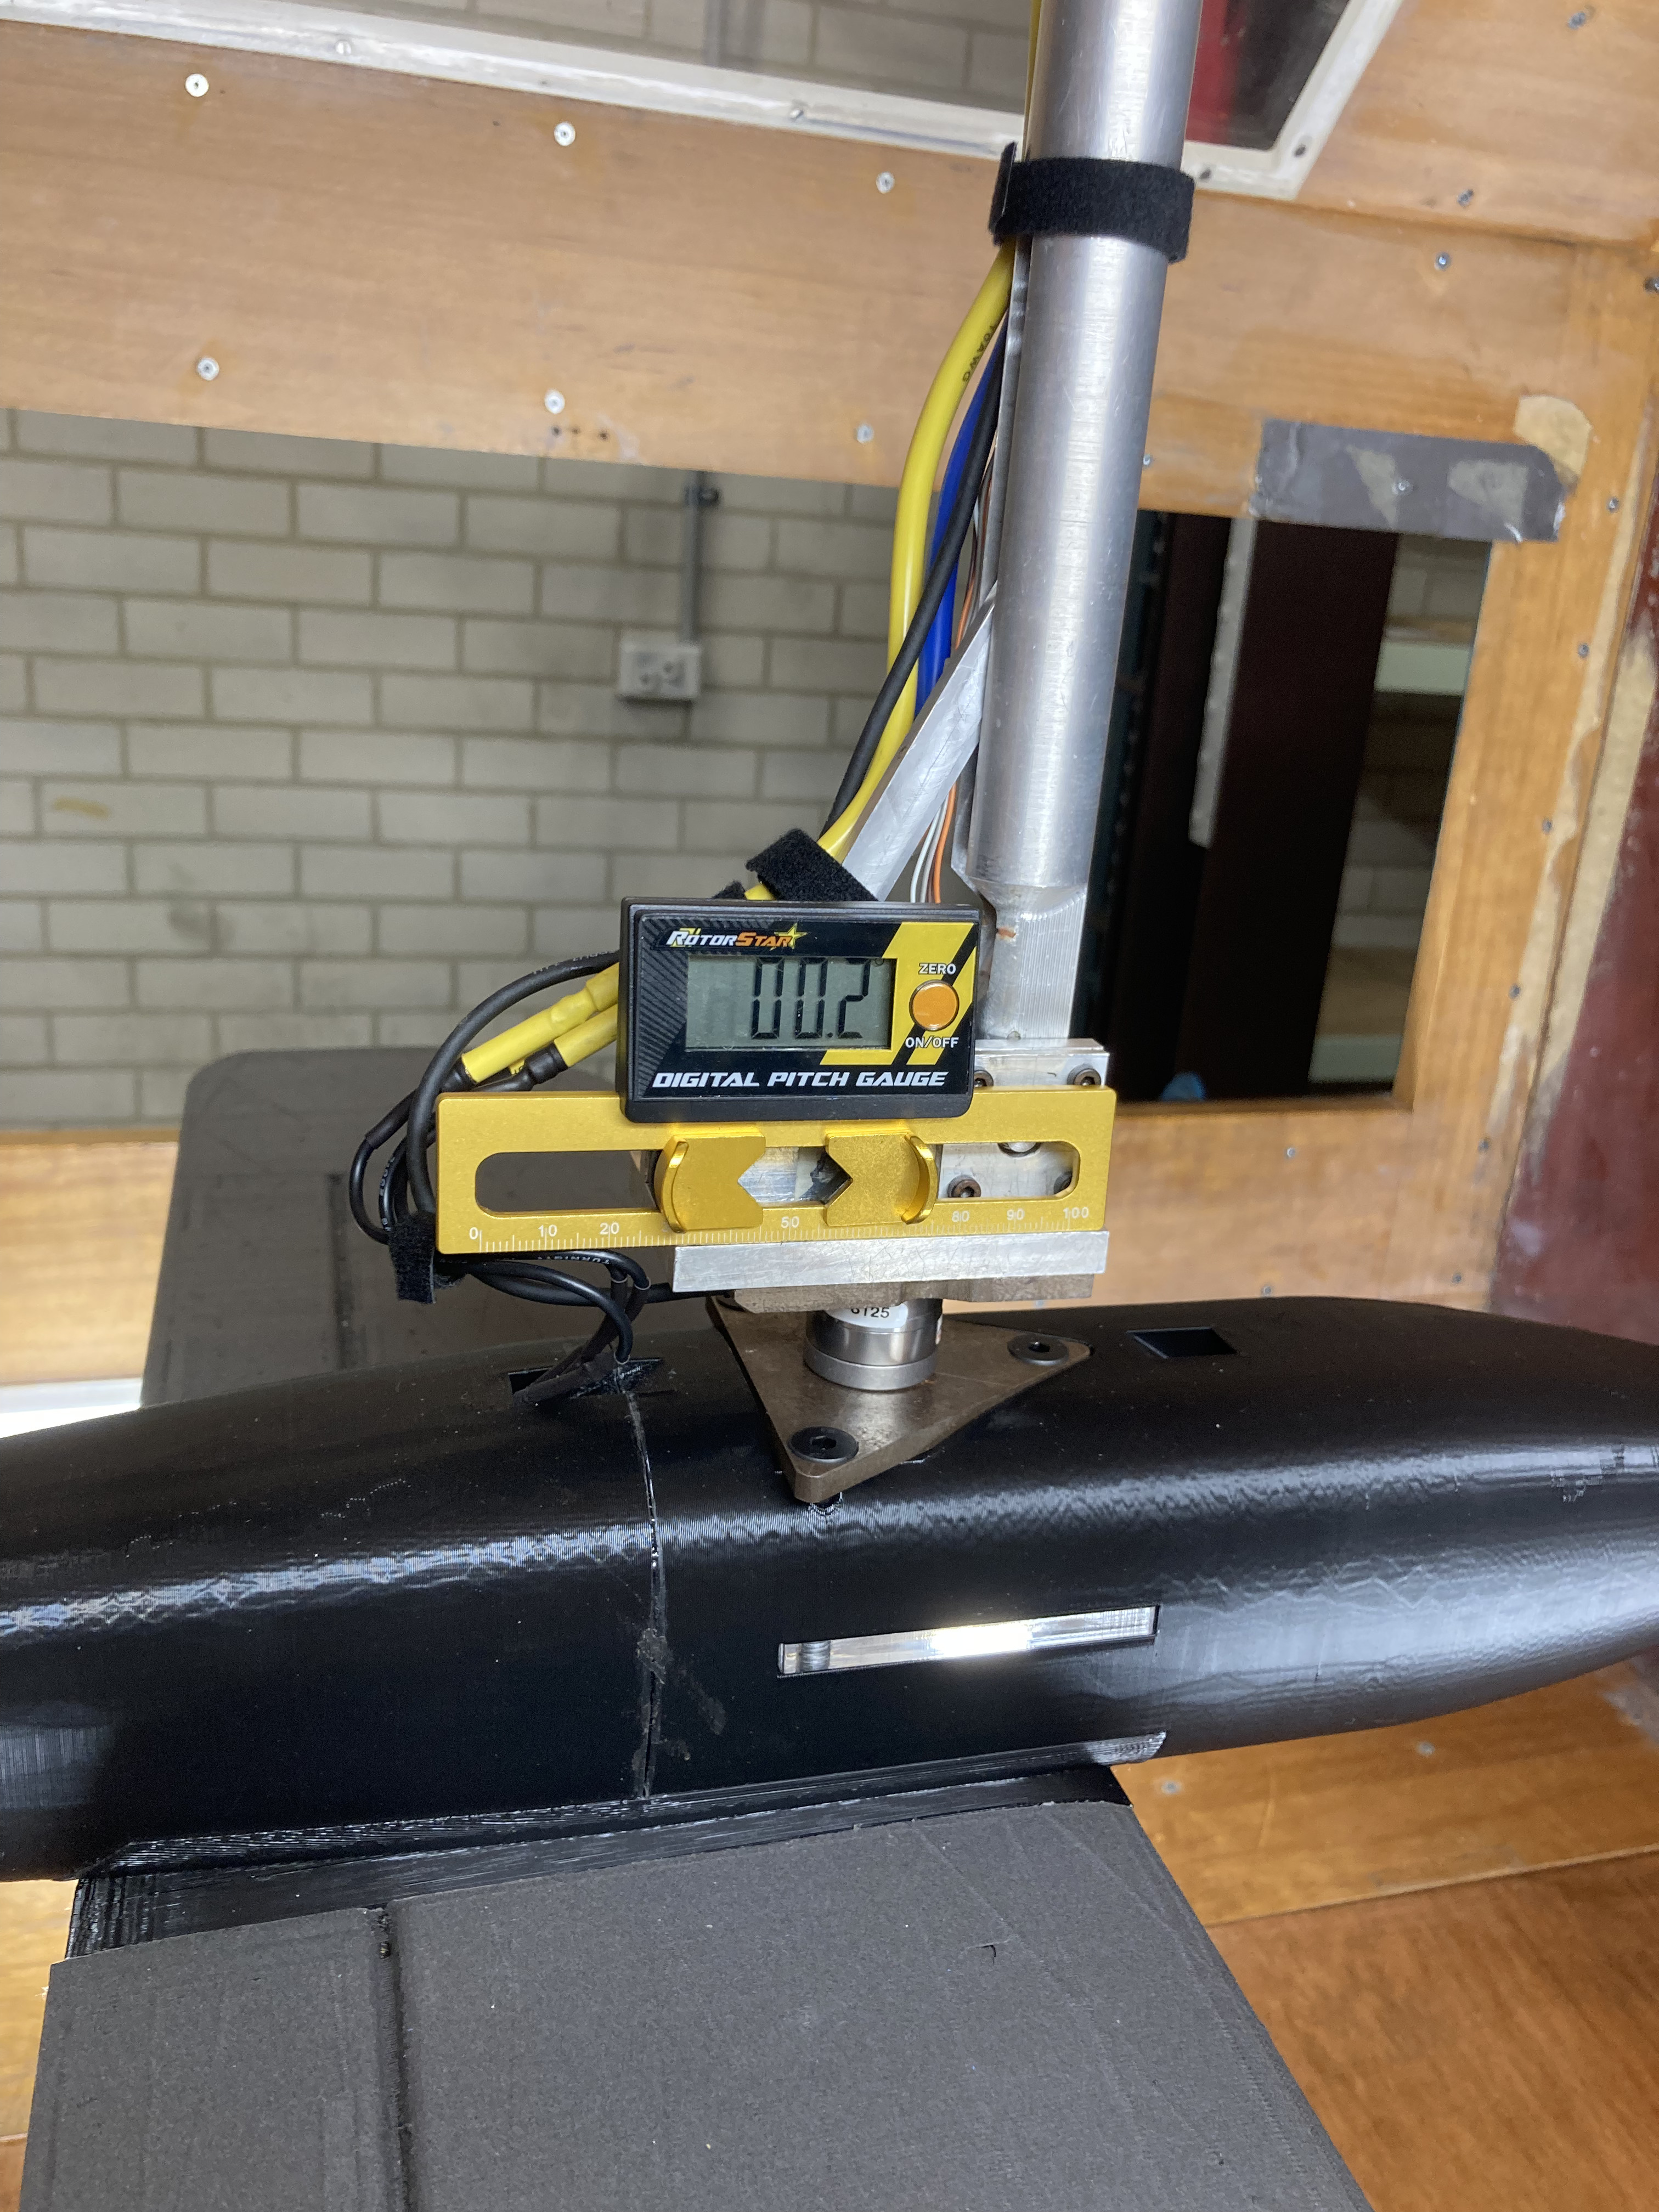
\includegraphics[scale=0.05]{04_Methodology/Figs/pitchGauge.jpg}
    \caption{Callibrating pitch of model mount to ensure \acrshort{AoA} is accurate}
    \label{fig:pitchGauge}
\end{figure}


When using the prop, the motor was supplied with a 7.4V battery, and the RPM was set to $\approx 6000 RPM$, $\approx 9000RPM$ and $\approx 11000 RPM$. The bias at each airspeed tested was first calculated to determine the change in forces and moments across the angles of attack tested. Following this, an \acrshort{AoA} sweep from -5$^{\circ}$ to 15$^{\circ}$ was undertaken for each airspeed analysed. For each velocity, the bias was recalculated. From the force and moment data collected, the main stability coefficients for the \acrshort{MAV} model could be determined.


\section{Stability Calculation}
To determine the stability in all the tested configurations, the stability derivatives of the model had to be determined. Data from the nano25 load cell was used to determine the loads and moments acting on the model about the mounting point. These values were transferred to the neutral point of the model at 20$\overline{c}$. The aerodynamic coefficients were determined using equations \ref{eqn:lift} to \ref{eqn:drag}, and the moment coefficients about the pitch, yaw and roll axis were calculated using Equations \ref{eqn:pitching} to \ref{eqn:sideslip}. 

%\todo{Add component list for MAV model in Wind Tunnel}

